\documentclass[11pt]{article}

\usepackage[utf8]{inputenc}
\usepackage[T1]{fontenc}
\usepackage[spanish]{babel}
\decimalpoint
\addto\captionsspanish{\renewcommand{\tablename}{Tabla}}
\usepackage{amsmath,amssymb}
\usepackage{graphicx}
\graphicspath{{../papers/paper_1_latent_geometry_full/}}
\usepackage{subcaption}
\usepackage{booktabs}
\usepackage[margin=1in]{geometry}
\usepackage{xurl}
\usepackage{hyperref}
\usepackage{xcolor}
\usepackage{float}

\hypersetup{
  colorlinks=true,
  linkcolor=blue,
  citecolor=blue,
  urlcolor=blue
}

\newcommand{\Enc}{\operatorname{Enc}}
\newcommand{\R}{\mathbb{R}}
\emergencystretch=3em

\title{Auditoría de la geometría molecular, temporal y evolutivo-taxonómica en representaciones latentes de AntigenLM para secuencias HA/NA de Influenza A}
\author{
Carlos Manuel Orrego-Franco\\
Juan Carlos Riaño-Rojas\\
\vspace{0.4em}
\small PCM Computational Applications Research Group\\
\small Universidad Nacional de Colombia\\
\small \texttt{corregof@unal.edu.co}; \texttt{jcrianoro@unal.edu.co}\\
\small ORCID: \url{https://orcid.org/0009-0001-9163-5137}
}
% TODO antes del envío: agregar el ORCID de Juan Carlos Riaño-Rojas si la revista objetivo lo requiere.
\date{\today}

\begin{document}
\maketitle

\begin{abstract}
Los modelos de lenguaje de secuencias se usan cada vez más como representaciones compactas de virus de rápida evolución, pero sus geometrías latentes deben auditarse antes de tratarlas como espacios de estados biológicos. Analizamos representaciones locales de AntigenLM almacenadas en caché para 111,756 registros HA/NA de Influenza~A de H1N1 y H3N2, representados como vectores de estados ocultos promediados en $\R^{384}$. Las correlaciones de Spearman dentro de subtipo muestran una fuerte organización molecular ($\rho = 0.8538$ en H1N1, $0.6678$ en H3N2 para distancia de Hamming HA+NA) y una débil correlación temporal global ($\rho = 0.0612$, $0.1540$), consistente con una población viral ramificada. Un control de embeddings aleatorios produce correlaciones de Hamming HA+NA cercanas a cero ($\rho = 0.0001$ en H1N1, $0.0004$ en H3N2), lo que indica que la señal molecular no es una consecuencia genérica de la geometría euclidiana aleatoria en alta dimensión. El PCA revela una fuerte concentración de varianza ($n_{95}=3$ global, razón de participación $1.91$), mientras que las estimaciones TwoNN después de deduplicación exacta HA+NA permanecen en un rango bajo de un solo dígito. Los vecindarios latentes locales están enriquecidos temporalmente después de la deduplicación: las diferencias temporales medianas entre vecinos más cercanos son de 2~meses frente a 42--43~meses para pares aleatorios H1N1 y 35~meses para pares aleatorios H3N2. El análisis de enriquecimiento por etiquetas de clado une la caché deduplicada con metadatos GISAID EpiFlu con 99.56\% de cobertura de unión y 92.63\% de cobertura con clado asignado y no marcado como no asignado. Para $k=5$, la precisión de clado de los vecinos latentes más cercanos es 0.9149 en H1N1 y 0.8609 en H3N2, lo que corresponde a enriquecimientos de 3.80 y 12.49 veces sobre líneas base aleatorias emparejadas por subtipo; la permutación de etiquetas de clado dentro de subtipo reduce la precisión a niveles de línea base aleatoria emparejada por subtipo. Las líneas base aleatorias estratificadas temporalmente atenúan el enriquecimiento, especialmente en H1N1 (1.55 veces en $\pm 6$~meses), mostrando que la coherencia de clado está parcialmente acoplada al recambio temporal de clados. En conjunto, la nube de embeddings de AntigenLM en caché está organizada molecularmente, es de baja dimensión bajo los diagnósticos evaluados, es localmente coherente en el tiempo y está enriquecida para etiquetas de clado evolutivo-taxonómicas, pero esta auditoría geométrica no establece similitud antigénica, preservación filogenética cuantitativa, relevancia para cepas vacunales, confiabilidad de generación de secuencias ni desempeño de pronóstico.
\end{abstract}

\section{Introducción}

El virus de Influenza A evoluciona mediante mutación, reasortamiento, selección inmune y cambios en el contexto epidemiológico. Las glicoproteínas de superficie hemaglutinina (HA) y neuraminidasa (NA) son centrales para la vigilancia porque moldean la entrada a la célula huésped, la liberación viral, la identidad de subtipo y la deriva antigénica. Sin embargo, la distancia molecular de secuencia, el fenotipo antigénico y el éxito evolutivo futuro son objetos distintos: la cartografía antigénica y los ensayos serológicos son necesarios para medir directamente la distancia antigénica, y la similitud de secuencia por sí sola no sustituye esos datos \cite{smith2004mapping,bedford2014integrating}. Antes de tratar cualquier representación aprendida como un espacio de estados para dinámicas evolutivas, sus propiedades geométricas deben auditarse directamente: ¿preserva la similitud molecular?, ¿es de baja dimensión bajo diagnósticos explícitos?, ¿muestra estructura relevante para la historia evolutiva? Estas son precondiciones, no sustitutos, para la validación biológica. Sustituciones específicas en HA pueden tener grandes efectos antigénicos \cite{koel2013substitutions}, lo que refuerza la necesidad de distinguir proxies moleculares de afirmaciones antigénicas.

Los modelos de lenguaje para secuencias biológicas ofrecen una vía atractiva para resumir grandes colecciones de secuencias virales. Los modelos de lenguaje de proteínas han mostrado que el entrenamiento no supervisado sobre secuencias puede codificar información estructural y funcional \cite{rives2021biological}, y los modelos de lenguaje de proteínas virales se han usado para estudiar escape evolutivo \cite{hie2021viral}. Modelos genómicos como DNABERT, Nucleotide Transformer y modelos de ADN de contexto largo extienden este programa de aprendizaje de representaciones a secuencias nucleotídicas \cite{ji2021dnabert,dallatorre2025nucleotide,nguyen2023hyenadna}. AntigenLM es un modelo de lenguaje de ADN reciente, enfocado en influenza y diseñado alrededor de la estructura de unidades funcionales y tareas de pronóstico HA/NA \cite{pei2026antigenlm}.

Antes de usar una representación aprendida como espacio de estados para dinámicas evolutivas, su geometría debe revisarse directamente. Un candidato útil a espacio de estados debería, como mínimo, organizar registros molecularmente similares, evitar colapsar en un artefacto ininterpretable de tiempo o composición de subtipo, y exhibir suficiente estructura de baja dimensión para hacer plausible el modelamiento posterior. Estos criterios son más débiles que una validación de pronóstico, pero son salvaguardas necesarias frente a tratar un embedding de alta dimensión como biológicamente significativo por simple afirmación.

Proponemos un marco reproducible de auditoría geométrica aplicable a cualquier modelo de lenguaje de secuencias virales antes de desplegarlo como espacio de estados biológico, y lo demostramos como estudio de caso sobre embeddings de AntigenLM para secuencias HA/NA de Influenza~A. Este artículo pregunta si estos embeddings satisfacen cuatro precondiciones mínimas: organización molecular, ausencia de colapso trivial por tiempo o subtipo, estructura de baja dimensión bajo diagnósticos explícitos y coherencia local con etiquetas evolutivo-taxonómicas de clado disponibles. No evaluamos validez antigénica, preservación cuantitativa de distancia filogenética ni desempeño de pronóstico. No reproducimos la tubería completa de entrenamiento o pronóstico de AntigenLM. El alcance es intencionalmente estrecho: la auditoría geométrica es un prerrequisito para trabajos más profundos, no un sustituto de ellos.

Operacionalmente, planteamos cinco preguntas descriptivas. Primero, ¿la distancia euclidiana latente sigue la distancia molecular de secuencia dentro de cada subtipo? Segundo, ¿la distancia latente se comporta como distancia cronológica, o la estructura temporal es principalmente local? Tercero, ¿qué tan concentrada está la varianza del embedding bajo PCA? Cuarto, ¿los diagnósticos locales de dimensión intrínseca concuerdan cualitativamente con la imagen lineal de PCA? Quinto, ¿los vecindarios de vecinos latentes más cercanos están enriquecidos para pertenencia a clados de GISAID más allá de líneas base aleatorias emparejadas por subtipo y estratificadas por tiempo? Intencionalmente no evaluamos generación de secuencias, optimización de mutaciones, inferencia de cepas vacunales ni pronóstico prospectivo.

\section{Métodos}

\subsection{Fuente de datos y alcance}

El análisis usa registros HA/NA de Influenza A procesados localmente y derivados de datos de GISAID \cite{shu2017gisaid}. Los registros se emparejaron por identificador de aislado durante el preprocesamiento y se retuvieron cuando HA, NA, subtipo, año y mes estaban disponibles después de filtros locales de calidad. La caché actual contiene 111,756 embeddings de registros recolectados entre 2000 y 2022: 46,125 H1N1 y 65,631 H3N2. Las secuencias completas no se imprimen en este manuscrito ni se redistribuyen en el paquete del artículo.

El análisis se limita a las representaciones HA/NA en caché y a metadatos agregados. Incluye anotaciones de clado de GISAID únicamente para una auditoría local de enriquecimiento de etiquetas después de la deduplicación. No incluye ensayos de inhibición de la hemaglutinación, títulos de neutralización, coordenadas de mapas antigénicos, árboles filogenéticos o distancias cuantitativas de árbol, estratificación geográfica, metadatos de huésped ni resultados prospectivos de pronóstico posteriores a 2022.

\subsection{Extracción local de embeddings}

Cada registro fue codificado con el checkpoint local de predicción de estilo AntigenLM \path{prediction_sequence/pytorch_model.bin} usando una envoltura local de modelo/tokenizador reconstruida a partir de archivos de configuración. El tokenizador representa nucleótidos a nivel de carácter y usa tokens estructurales para subtipo, HA, NA, separador, fin de secuencia y relleno. Para un registro $i$, la entrada tiene la forma
\[
\begin{aligned}
&\langle subtype\rangle \ \langle HA\rangle \ HA_i \ \langle sep\rangle \\
&\quad \langle NA\rangle \ NA_i \ \langle eos\rangle .
\end{aligned}
\]
El embedding es el promedio de los estados ocultos finales ponderado por la máscara de atención,
\[
z_i=\Enc_{\theta}(HA_i,NA_i)\in\R^{384}.
\]
Los metadatos de la caché registran el hash SHA256 del checkpoint
\path{6b942a0e2d6af0528a7307ff5754438ad55fdb97390297e9c0f11ffc9803dbff}, longitud máxima de secuencia 4000, tamaño de lote de embedding 4 y ausencia de entradas faltantes en la caché entre los registros procesados válidos. Por tanto, esta auditoría local debe leerse como un análisis de la representación en caché, no como una reproducción oficial de todos los procedimientos de inferencia o pronóstico de AntigenLM.

\subsection{Distancias y correlaciones con muestreo de pares}

La distancia latente entre los registros $i$ y $j$ es euclidiana:
\[
d_Z(i,j)=\lVert z_i-z_j\rVert_2.
\]
La distancia temporal es la separación absoluta de fecha de colección en meses,
\[
d_T(i,j)=\left|12(y_i-y_j)+(m_i-m_j)\right|.
\]
Para secuencias de segmento $x$ y $y$, la distancia de Hamming normalizada se calcula sobre el prefijo compartido cuando la diferencia de longitud es a lo sumo 5\% de la secuencia más larga:
\[
d_H(x,y)=\frac{1}{L}\sum_{\ell=1}^{L}\mathbf{1}\{x_\ell\neq y_\ell\},
\]
donde $L$ es la longitud más corta. Los pares que exceden la regla de tolerancia de longitud se omiten para ese cálculo de distancia molecular. La distancia de Hamming HA+NA es un promedio ponderado por longitud de las distancias de los segmentos HA y NA, con pesos dados por las longitudes más cortas de HA y NA en el par. Estas son proxies moleculares de distancia de secuencia. No son alineamientos biológicos curados ni distancias antigénicas.

Un panel focalizado de robustez también calculó distancias de Hamming nucleotídicas solo para NA y proxies simples de sensibilidad de Hamming sobre aminoácidos traducidos. Las cadenas de aminoácidos se obtuvieron por traducción en marco 0 de las cadenas nucleotídicas disponibles, con codones ambiguos mapeados a un símbolo de aminoácido desconocido y codones incompletos terminales descartados. Estas distancias traducidas se usan solo como análisis de sensibilidad. No deben interpretarse como alineamientos proteicos curados, validación a nivel de proteína, distancias de sitios antigénicos ni mediciones antigénicas.

Usando estas definiciones de distancia, calculamos correlaciones de rangos de Spearman entre distancias latentes y distancias moleculares o temporales mediante muestreo de pares específico por subtipo.

Las matrices completas de distancias de todos contra todos son inviables a esta escala. Por ello muestreamos 200,000 pares no idénticos por subtipo para cada una de tres semillas aleatorias (42, 7 y 123). Todo el muestreo de pares se realizó dentro de subtipo para evitar que la separación entre subtipos fuera la fuente dominante de correlación. Para cada conjunto muestreado, calculamos la correlación de rangos de Spearman \cite{spearman1904} entre $d_Z$ y $d_T$, la distancia de Hamming HA o la distancia de Hamming HA+NA. Resumimos medias y desviaciones estándar entre semillas a través de las tres semillas aleatorias; estas desviaciones estándar no son intervalos de confianza por bootstrap. Los valores p no se enfatizan porque las distancias por pares son dependientes y conteos muy grandes de pares muestreados pueden hacer que efectos despreciables parezcan estadísticamente significativos. La misma escala de muestreo de pares y las mismas semillas se reutilizaron después de la deduplicación exacta HA+NA en el panel de robustez.

\subsection{Deduplicación}

Los duplicados exactos son comunes en datos de vigilancia viral. Para TwoNN, los análisis locales de vecindarios temporales y las correlaciones de pares de robustez, eliminamos pares de secuencias HA+NA duplicados exactos reteniendo el primer representante de cada par HA+NA exacto encontrado en el orden de la caché. Esto dejó 82,306 registros: 36,753 H1N1 y 45,553 H3N2. La tabla principal de correlaciones con muestreo de pares usa la caché completa, y la tabla de robustez reporta correlaciones deduplicadas. Esta deduplicación elimina únicamente duplicados exactos del par de secuencias HA+NA; no elimina casi duplicados, registros duplicados en solo un segmento ni variantes nucleotídicas equivalentes a nivel de aminoácidos.

\subsection{Diagnósticos de dimensión efectiva: PCA y TwoNN}

El PCA se calculó a partir de la matriz de embeddings centrada usando el espectro exacto de covarianza \cite{jolliffe2002pca,jolliffe2016pca}. Reportamos $n_{80}$, $n_{90}$, $n_{95}$ y $n_{99}$, el número de componentes requeridos para explicar 80\%, 90\%, 95\% y 99\% de la varianza. También reportamos la razón de participación,
\[
PR=\frac{(\sum_i\lambda_i)^2}{\sum_i\lambda_i^2},
\]
donde $\lambda_i$ son autovalores positivos de la covarianza. La dimensión efectiva de PCA mide concentración lineal de varianza; no es idéntica a la dimensión intrínseca local ni a la dimensión de visualización.

Complementamos el espectro lineal de PCA con un diagnóstico local no lineal, TwoNN, para evaluar si la baja dimensión efectiva también es aparente bajo la geometría de vecinos más cercanos.

TwoNN estima dimensión intrínseca local a partir de razones entre distancias al segundo y al primer vecino más cercano \cite{facco2017intrinsic}. Para cada punto,
\[
\mu_i=\frac{r_{2,i}}{r_{1,i}},
\qquad
-\log(1-F_i)=d\log(\mu_i),
\]
donde $r_{1,i}$ y $r_{2,i}$ son distancias a vecinos más cercanos después de estandarizar las coordenadas del embedding, y $F_i$ es la distribución acumulada empírica de $\mu$. Evaluamos tamaños muestrales de 5,000, 10,000, 20,000 y 50,000 después de deduplicación exacta HA+NA, con semillas 42, 7 y 123 y niveles de recorte 0.01 y 0.05. El resultado se interpreta como un rango de sensibilidad, no como una dimensión exacta de variedad. Estimadores alternativos como los métodos de máxima verosimilitud de Levina-Bickel y DANCo se discuten como chequeos futuros de robustez \cite{levina2005maximum,ceruti2014danco}.

\subsection{Control de embeddings aleatorios}

Para evaluar si las correlaciones moleculares observadas son no triviales, generamos una línea base de embeddings aleatorios como control negativo. Para cada una de 10 réplicas, muestreamos independientemente para cada registro un vector de 384 dimensiones desde una distribución gaussiana estándar, $\mathcal{N}(0,I_{384})$, y normalizamos cada vector a norma $\ell_2$ unitaria antes de calcular distancias euclidianas. Este control evalúa geometría métrica aleatoria de alta dimensión independiente del contenido de secuencia HA/NA.

Para cada réplica aleatoria, calculamos correlaciones de Spearman entre distancias euclidianas en los embeddings aleatorios y distancias de Hamming HA+NA usando el mismo protocolo de muestreo de pares específico por subtipo que en el análisis principal de AntigenLM: 200,000 pares no idénticos solicitados por subtipo para cada semilla de muestreo 42, 7 y 123. Así, cada línea base aleatoria específica por subtipo resume 30 correlaciones: 10 réplicas de embeddings aleatorios por tres semillas de muestreo de pares. Si las correlaciones de AntigenLM surgieran solo de efectos métricos euclidianos genéricos en alta dimensión, se esperaría que la línea base aleatoria produjera correlaciones cercanas a cero.

\subsection{Vecindarios temporales locales}

Para cada subtipo después de deduplicación exacta HA+NA, calculamos vecinos euclidianos más cercanos en el espacio latente para $k=5,10,20$. Las coincidencias consigo mismo se excluyeron solicitando $k+1$ vecinos y removiendo el primer vecino retornado. Comparamos diferencias absolutas en índice mensual entre cada registro y sus $k$ vecinos latentes más cercanos contra pares aleatorios emparejados por subtipo con el mismo número de comparaciones. Como variante de control negativo, mantuvimos fijo el grafo de vecinos latentes pero permutamos las etiquetas de índice mensual de colección dentro de subtipo a través de tres semillas. Las líneas base aleatoria y de permutación de fechas controlan por distribuciones de fechas específicas de subtipo, pero no por todas las fuentes posibles de sesgo de muestreo, como geografía, huésped, intensidad de colección, composición de linajes o longitud de secuencia.

\subsection{Análisis de enriquecimiento por etiquetas de clado}

Para evaluar si la estructura de vecinos latentes más cercanos es coherente con anotaciones evolutivo-taxonómicas establecidas, unimos la caché de embeddings deduplicada exactamente por HA+NA con metadatos GISAID EpiFlu usando el identificador de aislado de GISAID (\path{epi_isl}/\path{Isolate_Id}) como llave de unión. Los metadatos se obtuvieron de cinco exportaciones XLS locales de GISAID EpiFlu que cubren registros recolectados entre 2000 y 2022 y se combinaron en una única tabla privada de metadatos asociada con \path{EPI_SET_260506bu}. Las etiquetas de clado anotadas como \path{unassigned} se trataron como valores faltantes y se excluyeron de los cálculos de precisión de clado, para evitar inflar métricas de coherencia con registros no anotados. No se redistribuyen con este manuscrito metadatos a nivel de accesión ni secuencias completas.

De los 82,306 registros deduplicados, 81,943 (99.56\%) se unieron exitosamente a metadatos GISAID. De estos registros deduplicados, 76,238 (92.63\%) tenían una etiqueta de clado no nula y no asignada como \path{unassigned}: 36,156 de 36,753 registros H1N1 (98.38\%) y 40,082 de 45,553 registros H3N2 (87.99\%). Los grafos de vecinos más cercanos para el análisis de clados se calcularon por separado dentro de cada subtipo usando distancias euclidianas en el espacio latente de 384 dimensiones.

Para cada registro consulta $i$ con etiqueta de clado asignada $c(i)$, calculamos la precisión de clado en $k$ como
\[
\operatorname{clade\text{-}precision@}k(i)=
\frac{1}{|V_i(k)|}\sum_{j\in V_i(k)}\mathbf{1}\{c(j)=c(i)\},
\]
donde $V_i(k)$ es el subconjunto de los $k$ vecinos latentes más cercanos de $i$ que también tienen etiqueta de clado asignada. Evaluamos $k\in\{5,10,20\}$, igualando el análisis local de vecindarios temporales.

Comparamos la precisión de clado contra tres controles. La línea base aleatoria global emparejada por subtipo muestrea $k$ registros con clado asignado del mismo subtipo, excluyendo el registro consulta, y promedia la precisión a través de las semillas 42, 7 y 123. Un control de permutación de etiquetas de clado mantiene fijo el grafo de vecinos latentes pero permuta las etiquetas de clado dentro de subtipo a través de 100 permutaciones replicadas. Finalmente, una línea base aleatoria estratificada temporalmente restringe los candidatos aleatorios a registros con clado asignado del mismo subtipo dentro de $\pm w$ meses del registro consulta, para $w\in\{6,12,24\}$ meses. Para este control temporal, la precisión verdadera de clado latente se recalcula sobre el mismo conjunto de consultas elegibles, porque algunos registros pueden tener menos de $k$ candidatos aleatorios con clado asignado dentro de una ventana estrecha.

Estas etiquetas de clado son anotaciones administrativas/evolutivas de GISAID basadas en prácticas de agrupamiento filogenético, no distancias filogenéticas cuantitativas ni mediciones antigénicas experimentales. El análisis evalúa la coherencia evolutivo-taxonómica local del embedding bajo las etiquetas de clado disponibles. No evalúa preservación filogenética proporcional a la distancia, similitud antigénica, escape inmune ni desempeño de pronóstico.

\section{Resultados}

\subsection{La distancia latente sigue la distancia molecular mucho más fuertemente que el tiempo global}

La caché contiene 111,756 embeddings en $\R^{384}$, que comprenden 46,125 registros H1N1 y 65,631 registros H3N2 recolectados entre 2000 y 2022 (Figura~\ref{fig:data-year}); la deduplicación exacta HA+NA retiene 82,306 registros para análisis de vecindarios y robustez (Figura~\ref{fig:lengths}).

\begin{figure}[H]
\centering
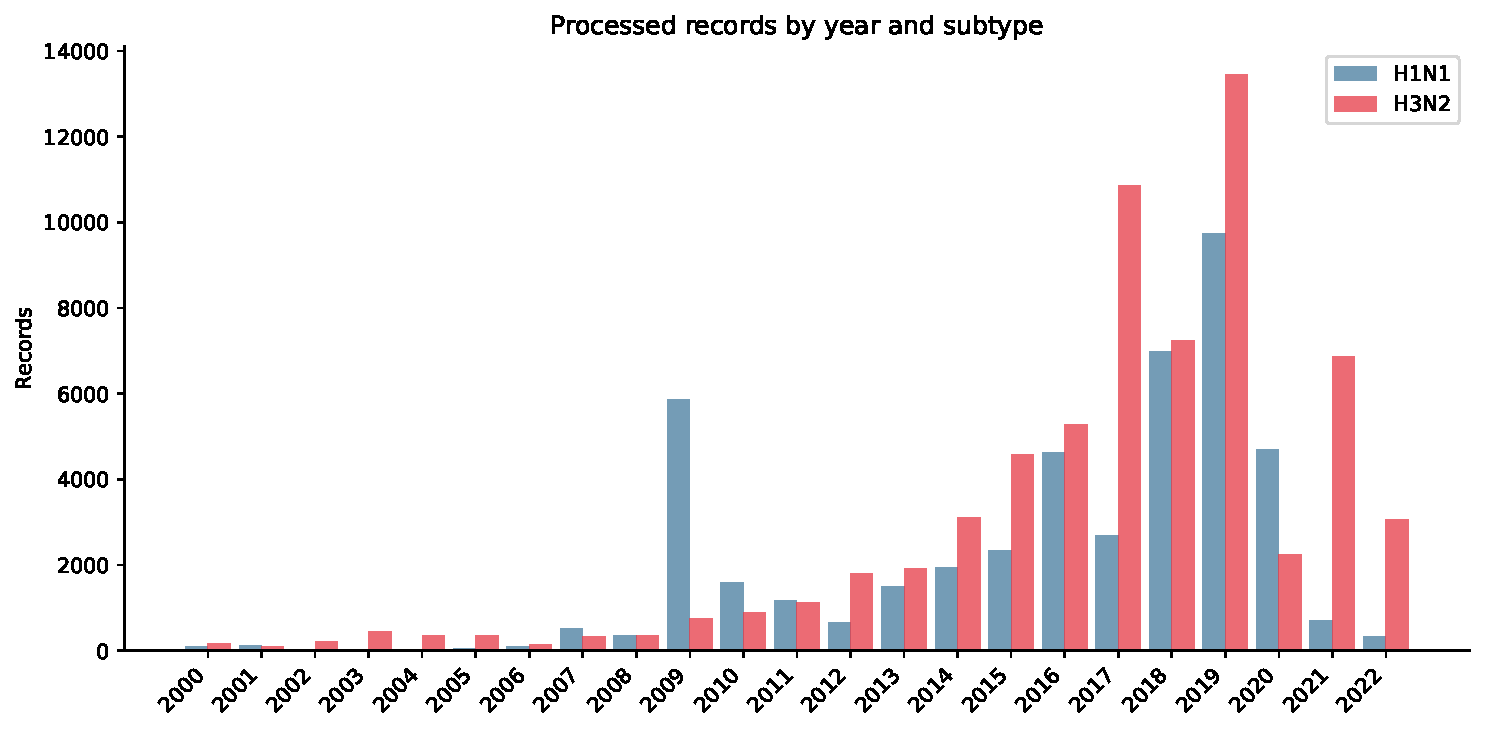
\includegraphics[width=0.78\textwidth]{figures/records_by_year_subtype.pdf}
\caption{Registros procesados por año y subtipo. Los conteos reflejan el conjunto local derivado de GISAID de HA/NA procesado y usado para construir la caché.}
\label{fig:data-year}
\end{figure}

\begin{figure}[H]
\centering
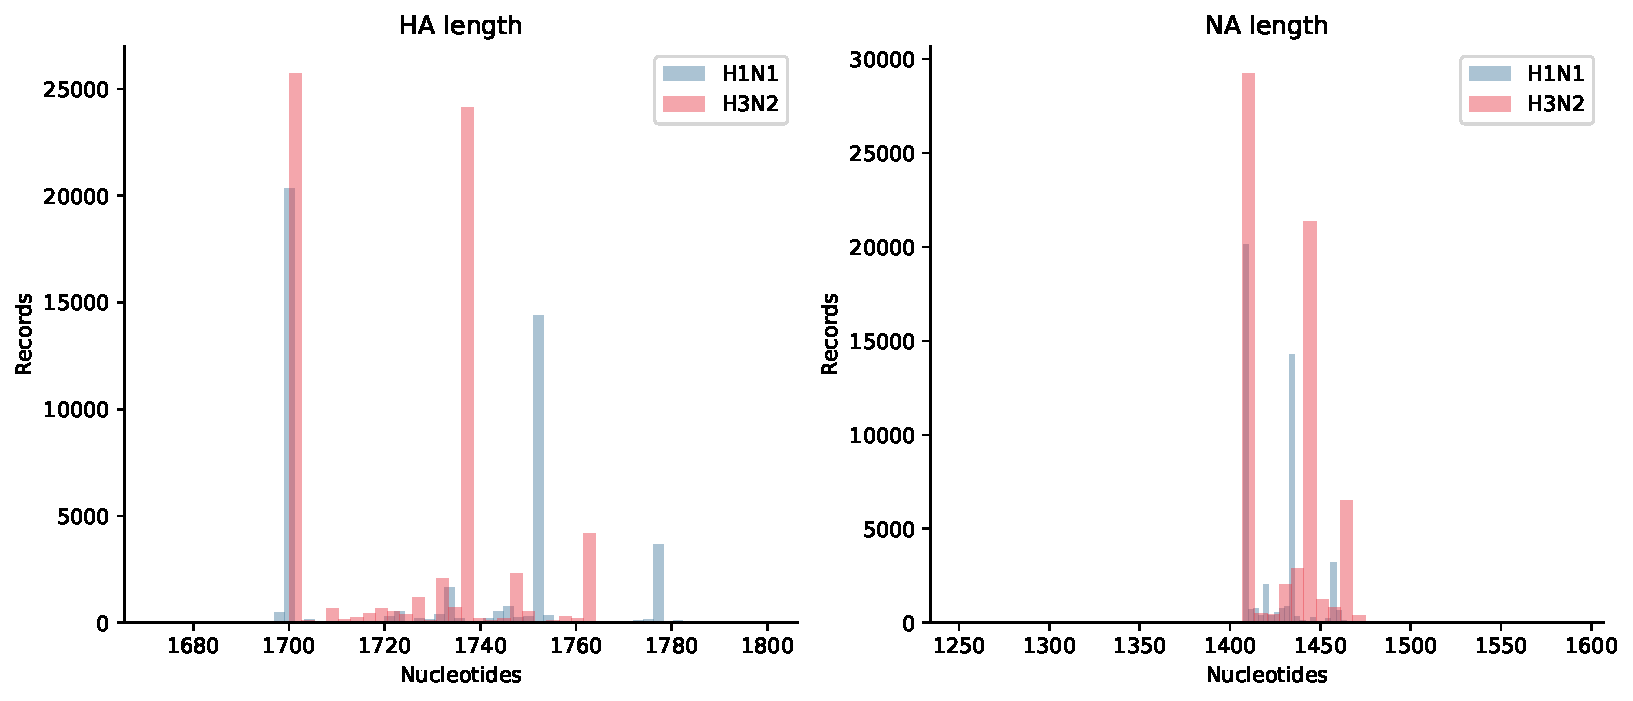
\includegraphics[width=0.82\textwidth]{figures/sequence_length_distributions.pdf}
\caption{Distribuciones de longitud de secuencia nucleotídica de HA y NA por subtipo después del preprocesamiento local y los filtros de calidad.}
\label{fig:lengths}
\end{figure}

Dentro de subtipo, la distancia euclidiana latente está fuertemente asociada con la distancia de Hamming nucleotídica, especialmente para el proxy combinado HA+NA (Tabla~\ref{tab:spearman}, Figura~\ref{fig:spearman}). Las correlaciones de Hamming HA+NA son 0.8538 para H1N1 y 0.6678 para H3N2. Las correlaciones solo con HA también son sustanciales: 0.8280 para H1N1 y 0.6082 para H3N2. Estos valores apoyan una afirmación de organización molecular para la geometría local del embedding.

En contraste, las correlaciones con la separación temporal absoluta son débiles: 0.0612 para H1N1 y 0.1540 para H3N2. Esto no implica ausencia de estructura evolutiva. No debería esperarse que una población viral ramificada, con reasortamiento y muestreo espacial, se ubique sobre una sola línea cronológica en distancia euclidiana latente. La pregunta más relevante para el modelamiento local posterior es si los vecindarios, en lugar de todos los pares, son temporalmente coherentes.

\begin{table}[H]
\centering
\caption{Correlaciones de Spearman con muestreo de pares entre distancia euclidiana latente y proxies temporales o moleculares de distancia de secuencia. Los valores resumen tres semillas aleatorias de muestreo de pares, con 200,000 pares solicitados por subtipo y semilla; las desviaciones estándar reportadas son desviaciones entre semillas, no intervalos de confianza. Los pares moleculares pueden omitirse cuando falla la regla de tolerancia de longitud.}
\label{tab:spearman}
\begin{tabular}{llrrr}
\toprule
Métrica & Subtipo & media $\rho$ & sd $\rho$ & pares válidos \\
\midrule
Distancia temporal & H1N1 & 0.0612 & 0.0009 & 200000 \\
Distancia temporal & H3N2 & 0.1540 & 0.0008 & 200000 \\
Hamming HA & H1N1 & 0.8280 & 0.0009 & 199914 \\
Hamming HA & H3N2 & 0.6082 & 0.0005 & 199989 \\
Hamming HA+NA & H1N1 & 0.8538 & 0.0006 & 199903 \\
Hamming HA+NA & H3N2 & 0.6678 & 0.0014 & 199538 \\
\bottomrule
\end{tabular}
\end{table}

\begin{figure}[H]
\centering
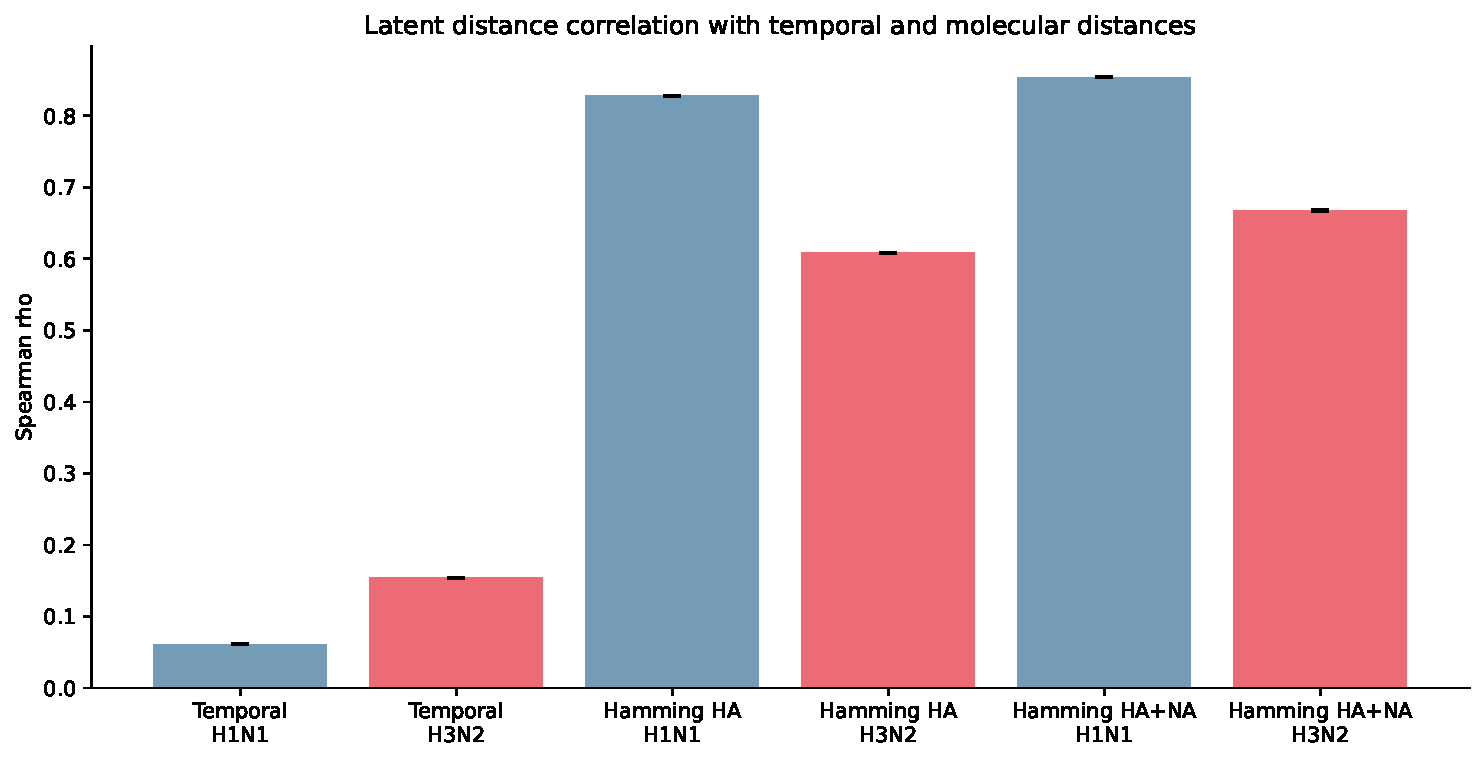
\includegraphics[width=0.85\textwidth]{figures/spearman_latent_vs_distances.pdf}
\caption{Resumen de correlaciones de Spearman para distancia euclidiana latente frente a proxies temporales y moleculares de distancia de secuencia. Las correlaciones se calculan dentro de subtipo y se resumen a través de semillas aleatorias de muestreo de pares.}
\label{fig:spearman}
\end{figure}

\subsection{Los embeddings aleatorios no reproducen la señal molecular}

El control negativo de embeddings aleatorios produce correlaciones de Hamming HA+NA cercanas a cero en ambos subtipos (Tabla~\ref{tab:random-baseline}). A través de 10 réplicas de embeddings aleatorios y tres semillas de muestreo de pares, la correlación media de la línea base aleatoria es 0.0001 para H1N1 y 0.0004 para H3N2. Las correlaciones correspondientes de AntigenLM son 0.8538 y 0.6678, respectivamente.

Este resultado muestra que la organización molecular detectada en las distancias latentes de AntigenLM no es una consecuencia trivial de calcular distancias euclidianas entre vectores aleatorios de 384 dimensiones. La variación entre semillas y entre réplicas en la línea base aleatoria es pequeña (desviación estándar 0.0019--0.0021), consistente con un control negativo estable de señal cero.

\begin{table}[H]
\centering
\caption{Línea base de embeddings aleatorios para correlaciones de Hamming HA+NA. Los embeddings aleatorios son vectores gaussianos de 384 dimensiones normalizados a norma $\ell_2$ unitaria. Los valores resumen 10 réplicas de embeddings aleatorios y tres semillas de muestreo de pares por réplica, usando el mismo protocolo específico por subtipo que en la Tabla~\ref{tab:spearman}.}
\label{tab:random-baseline}
\begin{tabular}{lrrrr}
\toprule
Métrica & Subtipo & media $\rho$ aleatoria & sd $\rho$ aleatoria & media $\rho$ AntigenLM \\
\midrule
Hamming HA+NA & H1N1 & 0.0001 & 0.0019 & 0.8538 \\
Hamming HA+NA & H3N2 & 0.0004 & 0.0021 & 0.6678 \\
\bottomrule
\end{tabular}
\end{table}

\subsection{Los vecindarios latentes están enriquecidos para pertenencia a clados de GISAID}

La unión de la caché deduplicada exactamente por HA+NA con metadatos GISAID EpiFlu mediante identificador de aislado alcanzó 99.56\% de cobertura, con 92.63\% de los registros deduplicados portando una etiqueta de clado asignada y no marcada como no asignada (Tabla~\ref{tab:clade-coverage}). La alta tasa de unión indica que la exportación de metadatos captura esencialmente el mismo universo de registros que la caché deduplicada de embeddings. La cobertura es mayor en H1N1 (98.38\% de cobertura con clado asignado) que en H3N2 (87.99\%), y esta diferencia entre subtipos se considera de nuevo en las limitaciones.

\begin{table}[H]
\centering
\caption{Cobertura de etiquetas de clado de GISAID después de unir la caché deduplicada exactamente por HA+NA con metadatos GISAID EpiFlu mediante identificador de aislado. Los registros con \texttt{Clade = unassigned} se tratan como faltantes.}
\label{tab:clade-coverage}
\begin{tabular}{lrrrrr}
\toprule
Grupo & n caché & n unidos & unión \% & n clado asignado & clado asignado \% \\
\midrule
H1N1 & 36,753 & 36,723 & 99.92 & 36,156 & 98.38 \\
H3N2 & 45,553 & 45,220 & 99.27 & 40,082 & 87.99 \\
Combinado & 82,306 & 81,943 & 99.56 & 76,238 & 92.63 \\
\bottomrule
\end{tabular}
\end{table}

La precisión de clado en $k$ es sustancialmente mayor para vecinos latentes que para registros aleatorios emparejados por subtipo en ambos subtipos (Tabla~\ref{tab:clade-enrichment}, Figura~\ref{fig:clade-enrichment}). Para H1N1 en $k=5$, los vecinos latentes comparten el clado de consulta en 91.49\% de los casos, comparado con una línea base aleatoria emparejada por subtipo de 24.09\%, un enriquecimiento de 3.80 veces. Para H3N2 en $k=5$, la precisión es 86.09\% frente a una línea base aleatoria emparejada por subtipo de 6.89\%, un enriquecimiento de 12.49 veces. El enriquecimiento disminuye solo modestamente al aumentar $k$ de 5 a 20, lo cual es esperable porque los vecindarios se expanden para incluir vecinos latentes más distantes.

La mayor razón de enriquecimiento en H3N2 refleja la granularidad más fina de las etiquetas de clado H3N2 en esta exportación de metadatos: la línea base aleatoria emparejada por subtipo es baja porque las etiquetas están distribuidas entre más clados. H1N1 tiene una línea base aleatoria emparejada por subtipo más alta porque sus clados asignados son más amplios y desbalanceados, pero su precisión absoluta de clado latente es ligeramente mayor. En ambos subtipos, el control de permutación de etiquetas de clado reduce la precisión al rango de la línea base aleatoria global emparejada por subtipo, lo que indica que la coherencia de clado observada depende de las asignaciones reales de clado y no solo de la distribución marginal de clados.

\begin{table}[H]
\centering
\caption{Precisión de clado en $k$ para vecinos latentes más cercanos frente a controles aleatorios emparejados por subtipo y de permutación de etiquetas de clado. Solo se incluyen como consultas registros con etiquetas de clado asignadas y no marcadas como no asignadas; los vecinos sin etiqueta de clado asignada se excluyen del denominador de precisión.}
\label{tab:clade-enrichment}
\begin{tabular}{lrrrr}
\toprule
Subtipo & k & precisión@k & aleatorio por subtipo & enriquecimiento \\
\midrule
H1N1 & 5 & 0.9149 & 0.2409 & 3.80$\times$ \\
H1N1 & 10 & 0.8933 & 0.2403 & 3.72$\times$ \\
H1N1 & 20 & 0.8647 & 0.2404 & 3.60$\times$ \\
H3N2 & 5 & 0.8609 & 0.0689 & 12.49$\times$ \\
H3N2 & 10 & 0.8325 & 0.0689 & 12.08$\times$ \\
H3N2 & 20 & 0.7927 & 0.0688 & 11.51$\times$ \\
\bottomrule
\end{tabular}
\end{table}

\begin{figure}[H]
\centering
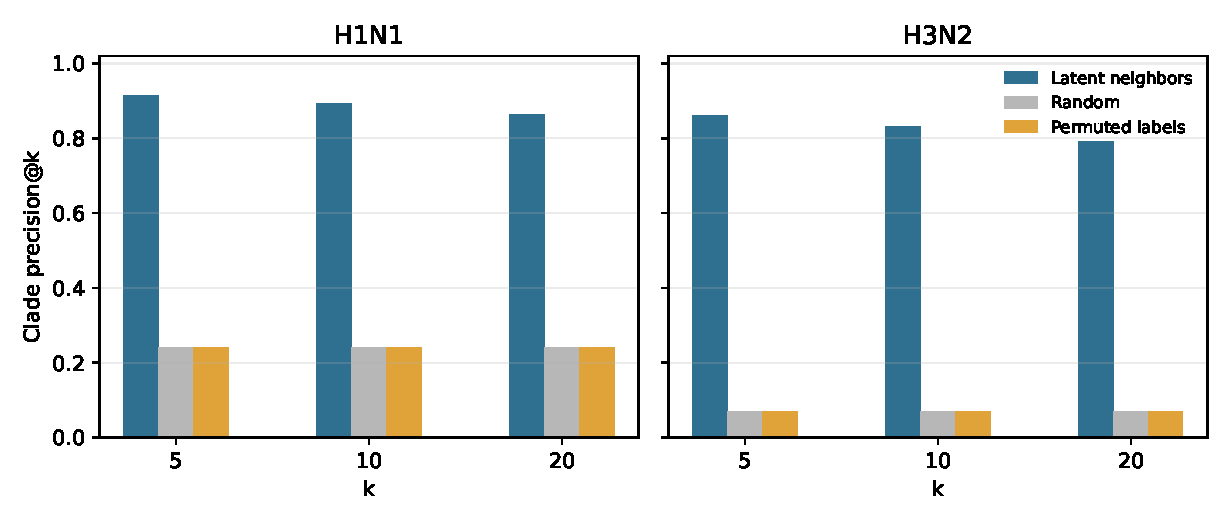
\includegraphics[width=0.86\textwidth]{figures/clade_precision_enrichment.pdf}
\caption{Precisión de clado en $k$ para vecinos latentes más cercanos comparada con registros aleatorios emparejados por subtipo y controles de permutación de etiquetas de clado dentro de subtipo. El grafo fijo de vecinos latentes se calcula por separado dentro de subtipo después de deduplicación exacta HA+NA.}
\label{fig:clade-enrichment}
\end{figure}

Dado que los clados están estructurados temporalmente, las líneas base aleatorias emparejadas por subtipo por sí solas pueden sobreestimar la independencia de la coherencia de clado respecto al calendario. Por ello, las líneas base aleatorias estratificadas temporalmente restringen los candidatos aleatorios a registros con clado asignado del mismo subtipo dentro de $\pm 6$, $\pm 12$ o $\pm 24$ meses de la consulta. Este control eleva sustancialmente la línea base aleatoria estratificada, especialmente en H1N1 (Tabla~\ref{tab:clade-temporal-stratified}). Para $k=5$ y $\pm 6$ meses, el enriquecimiento de H1N1 se reduce a 1.55 veces, mientras que H3N2 permanece enriquecido 3.18 veces. Así, la coherencia de clado está parcialmente acoplada al recambio temporal de clados, particularmente en H1N1. No obstante, el resultado permanece por encima de la línea base aleatoria estratificada por tiempo en todas las ventanas evaluadas, apoyando una afirmación cautelosa de coherencia evolutivo-taxonómica local, no una afirmación de estructura filogenética independiente del tiempo.

\begin{table}[H]
\centering
\caption{Sensibilidad de estratificación temporal para precisión de clado@5. Los candidatos aleatorios son registros con clado asignado del mismo subtipo dentro de la ventana declarada de mes de colección; la precisión latente verdadera se recalcula sobre el mismo conjunto de consultas elegibles. La precisión latente verdadera de clado es constante entre tamaños de ventana para un subtipo dado; solo la línea base aleatoria estratificada y la razón de enriquecimiento varían con el ancho de ventana.}
\label{tab:clade-temporal-stratified}
\small
\begin{tabular}{lrrrrr}
\toprule
Subtipo & ventana & prec. verdadera & aleatorio estrat. & enriq. & consultas \\
\midrule
H1N1 & $\pm 6$ meses & 0.9149 & 0.5892 & 1.55$\times$ & 36,156 \\
H1N1 & $\pm 12$ meses & 0.9149 & 0.5405 & 1.69$\times$ & 36,156 \\
H1N1 & $\pm 24$ meses & 0.9149 & 0.4681 & 1.95$\times$ & 36,156 \\
H3N2 & $\pm 6$ meses & 0.8610 & 0.2707 & 3.18$\times$ & 40,080 \\
H3N2 & $\pm 12$ meses & 0.8610 & 0.2288 & 3.76$\times$ & 40,080 \\
H3N2 & $\pm 24$ meses & 0.8609 & 0.1548 & 5.56$\times$ & 40,081 \\
\bottomrule
\end{tabular}
\normalsize
\end{table}

Estos resultados extienden el hallazgo de organización molecular: el embedding no solo preserva estructura de distancia de secuencia nucleotídica bajo proxies de Hamming, sino que también organiza vecindarios locales de acuerdo con anotaciones de clado establecidas por GISAID. Esta es una auditoría biológica con anotación externa más fuerte que la preservación de distancia de Hamming por sí sola, porque la pertenencia a clado refleja agrupamiento evolutivo-taxonómico y no solo similitud cruda por pares de secuencia. La interpretación sigue siendo acotada: esto es enriquecimiento por etiquetas de clado, no evidencia de preservación filogenética cuantitativa, similitud antigénica, escape inmune ni desempeño de pronóstico.

\subsection{El PCA muestra una fuerte concentración lineal de varianza}

El espectro global de embeddings está altamente concentrado (Tabla~\ref{tab:pca}, Figura~\ref{fig:pca-spectrum}). Dos componentes explican al menos 90\% de la varianza global, tres explican al menos 95\% y 10 explican al menos 99\%. La razón de participación global es 1.91. Los espectros específicos por subtipo también están concentrados, con H1N1 alcanzando 95\% de varianza en tres componentes y H3N2 en cinco componentes.

Este resultado debe interpretarse como fuerte anisotropía y baja dimensión efectiva lineal. Por sí solo, no prueba que los datos estén sobre una variedad biológica suave de baja dimensión. Los primeros componentes principales pueden reflejar una mezcla de direcciones moleculares, específicas de subtipo, temporales, de densidad de muestreo e inducidas por el modelo.

\begin{table}[H]
\centering
\caption{Dimensión efectiva por PCA de los embeddings de AntigenLM. $n_q$ denota el número de componentes principales requeridos para explicar la fracción $q$ de varianza; PR es la razón de participación del espectro de covarianza.}
\label{tab:pca}
\begin{tabular}{lrrrrrr}
\toprule
Grupo & n & $n_{80}$ & $n_{90}$ & $n_{95}$ & $n_{99}$ & PR \\
\midrule
global & 111,756 & 2 & 2 & 3 & 10 & 1.91 \\
H1N1 & 46,125 & 1 & 2 & 3 & 11 & 1.43 \\
H3N2 & 65,631 & 1 & 3 & 5 & 16 & 1.53 \\
\bottomrule
\end{tabular}
\end{table}

\begin{figure}[H]
\centering
\begin{subfigure}{0.48\textwidth}
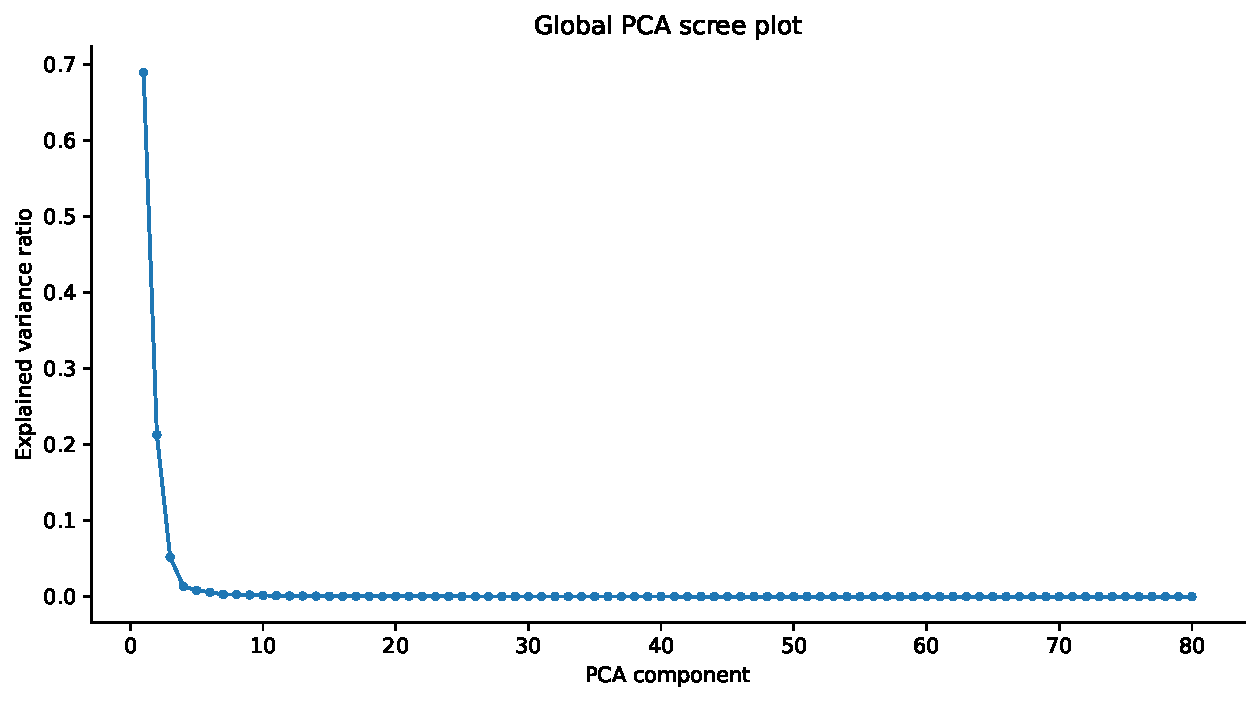
\includegraphics[width=\textwidth]{figures/pca_scree_global.pdf}
\caption{Gráfico scree global.}
\end{subfigure}
\begin{subfigure}{0.48\textwidth}
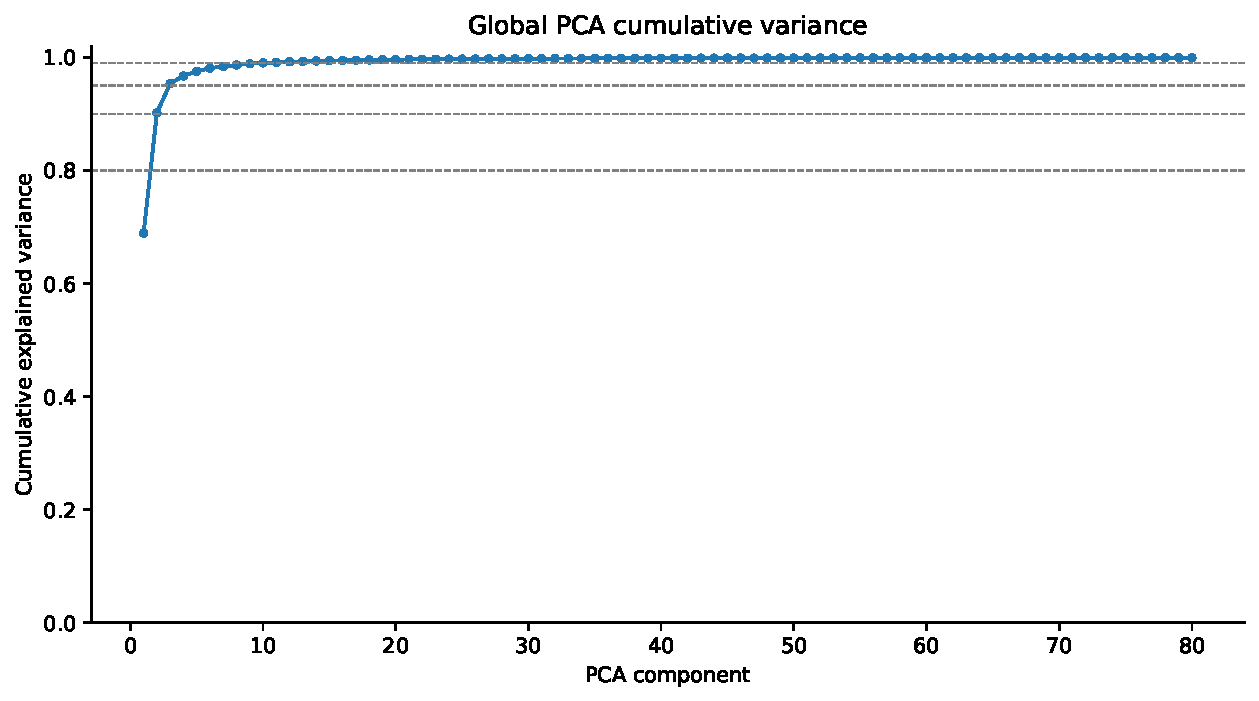
\includegraphics[width=\textwidth]{figures/pca_cumulative_global.pdf}
\caption{Varianza acumulada global.}
\end{subfigure}
\caption{Espectro global de PCA. El espectro está fuertemente concentrado, lo que apoya baja dimensión efectiva lineal pero no establece dimensión intrínseca de variedad.}
\label{fig:pca-spectrum}
\end{figure}

\begin{figure}[H]
\centering
\begin{subfigure}{0.48\textwidth}
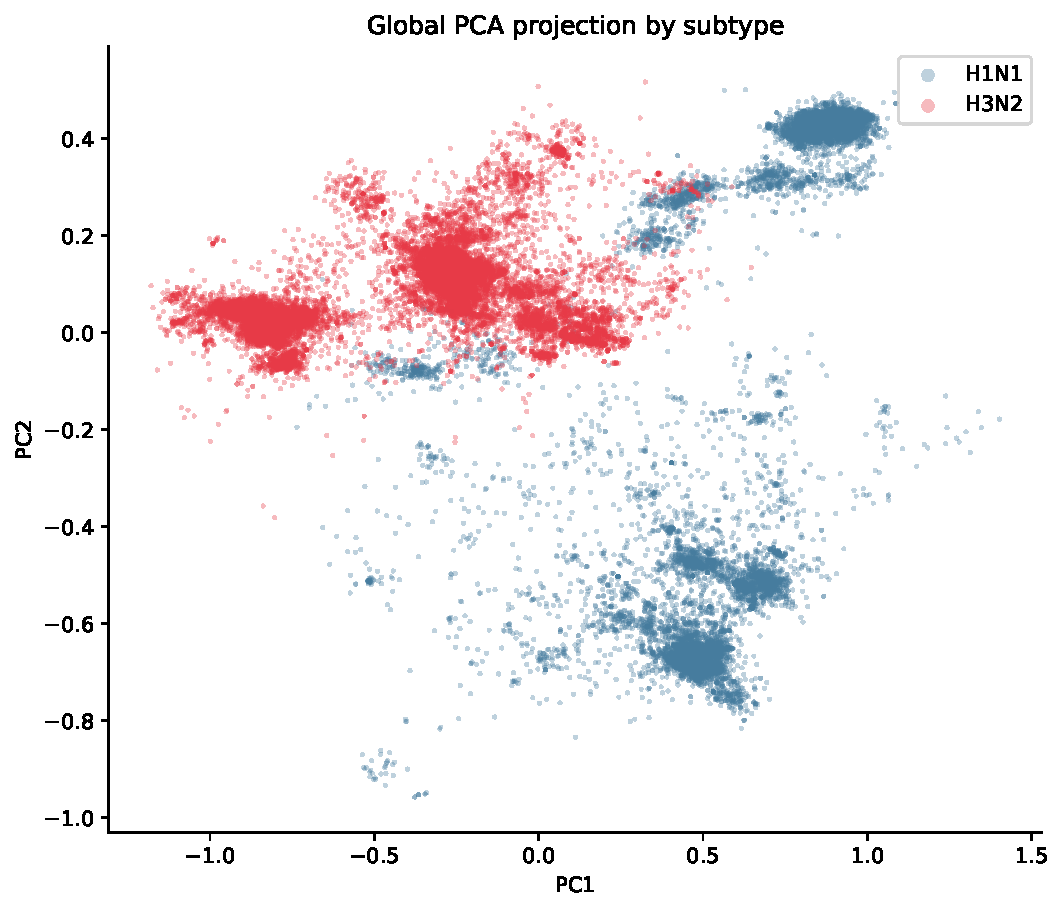
\includegraphics[width=\textwidth]{figures/pca_2d_by_subtype.pdf}
\caption{Coloreado por subtipo.}
\end{subfigure}
\begin{subfigure}{0.48\textwidth}
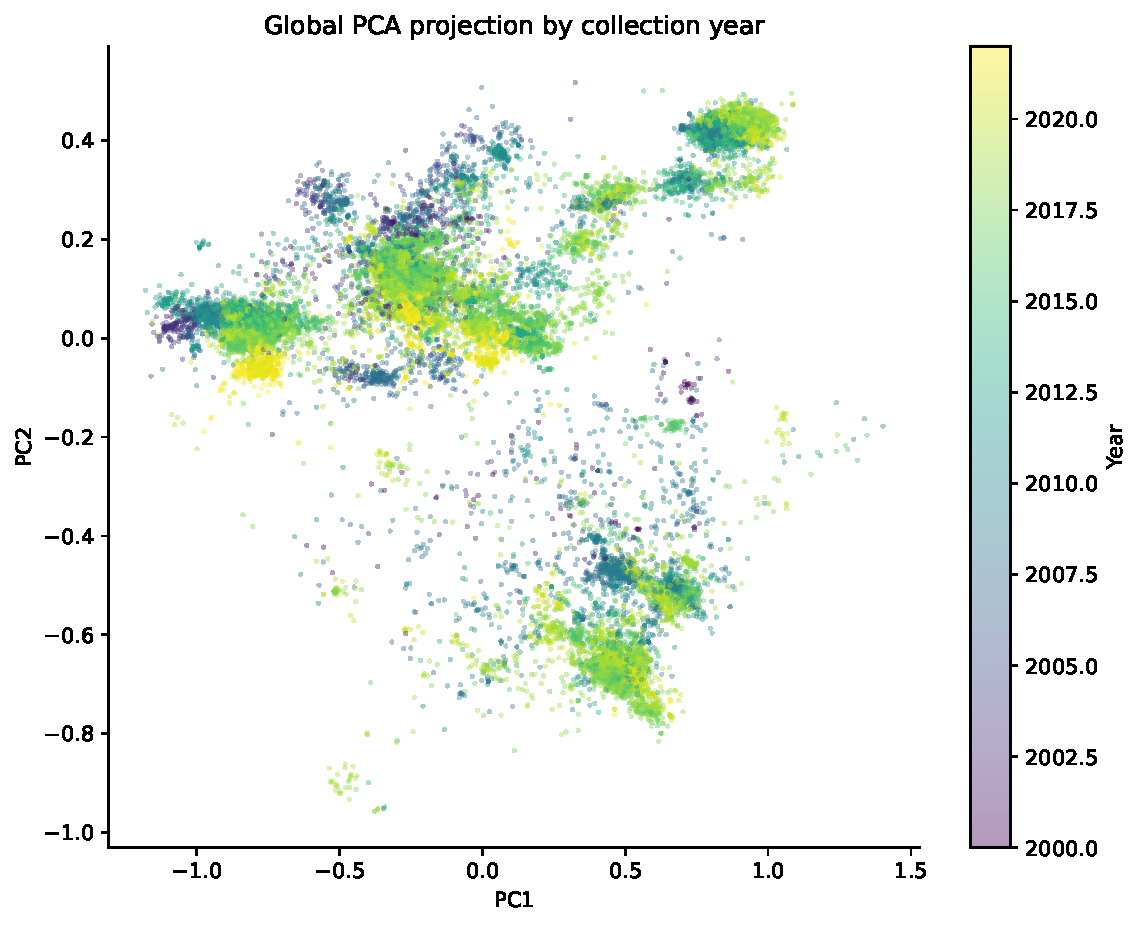
\includegraphics[width=\textwidth]{figures/pca_2d_by_year.pdf}
\caption{Coloreado por año.}
\end{subfigure}
\caption{Proyección PCA global en dos dimensiones. La proyección es descriptiva y no debe leerse como una representación completa de relaciones evolutivas o antigénicas. En particular, esta vista bidimensional no constituye evidencia filogenética cuantitativa, antigénica ni de pronóstico.}
\label{fig:pca-2d}
\end{figure}

\subsection{Las estimaciones TwoNN son bajas pero sensibles al recorte}

TwoNN proporciona un diagnóstico local de vecinos más cercanos que complementa el espectro lineal de PCA. Después de deduplicación exacta HA+NA, la dimensión estimada permanece estable a través de tamaños muestrales pero cambia con el nivel de recorte (Tabla~\ref{tab:twonn}, Figura~\ref{fig:twonn}). Con recorte 0.01, las estimaciones son aproximadamente 3.85--3.90; con recorte 0.05, son aproximadamente 5.40--5.50. Los valores medios de $R^2$ están cerca de 0.97--0.98.

La conclusión clave no es una única dimensión exacta. Más bien, PCA y TwoNN concuerdan cualitativamente en que la representación nominal de 384 dimensiones tiene una estructura efectiva mucho menor bajo las opciones de preprocesamiento evaluadas. La sensibilidad al recorte es informativa: las estimaciones de dimensión intrínseca deben reportarse como diagnósticos con supuestos, no como constantes biológicas fijas.

\begin{table}[H]
\centering
\caption{Sensibilidad de dimensión intrínseca TwoNN después de deduplicación exacta HA+NA. Los valores resumen tres semillas aleatorias para cada tamaño muestral y nivel de recorte.}
\label{tab:twonn}
\begin{tabular}{rrrr}
\toprule
Tamaño muestral & recorte & media dimensión & media $R^2$ \\
\midrule
5,000 & 0.01 & 3.89 & 0.981 \\
5,000 & 0.05 & 5.50 & 0.972 \\
10,000 & 0.01 & 3.88 & 0.978 \\
10,000 & 0.05 & 5.49 & 0.972 \\
20,000 & 0.01 & 3.85 & 0.978 \\
20,000 & 0.05 & 5.45 & 0.971 \\
50,000 & 0.01 & 3.90 & 0.980 \\
50,000 & 0.05 & 5.40 & 0.970 \\
\bottomrule
\end{tabular}
\end{table}

\begin{figure}[H]
\centering
\begin{subfigure}{0.48\textwidth}
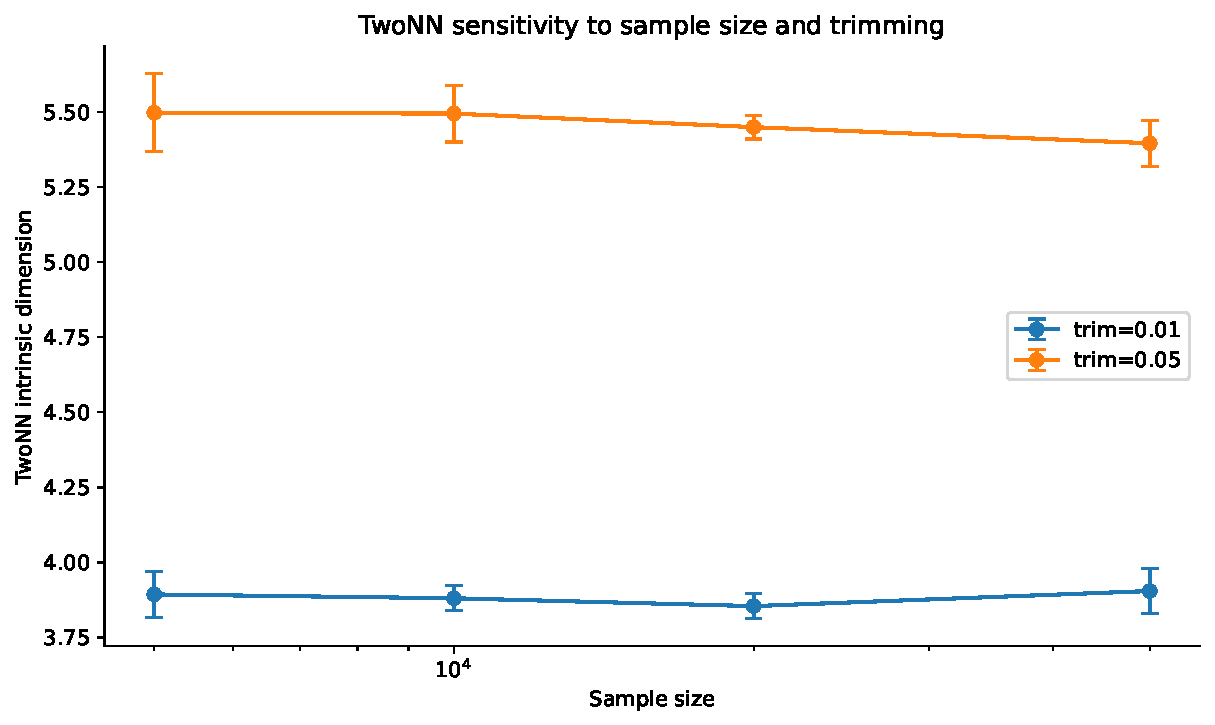
\includegraphics[width=\textwidth]{figures/twonn_sensitivity.pdf}
\caption{Sensibilidad a tamaño muestral y recorte.}
\end{subfigure}
\begin{subfigure}{0.48\textwidth}
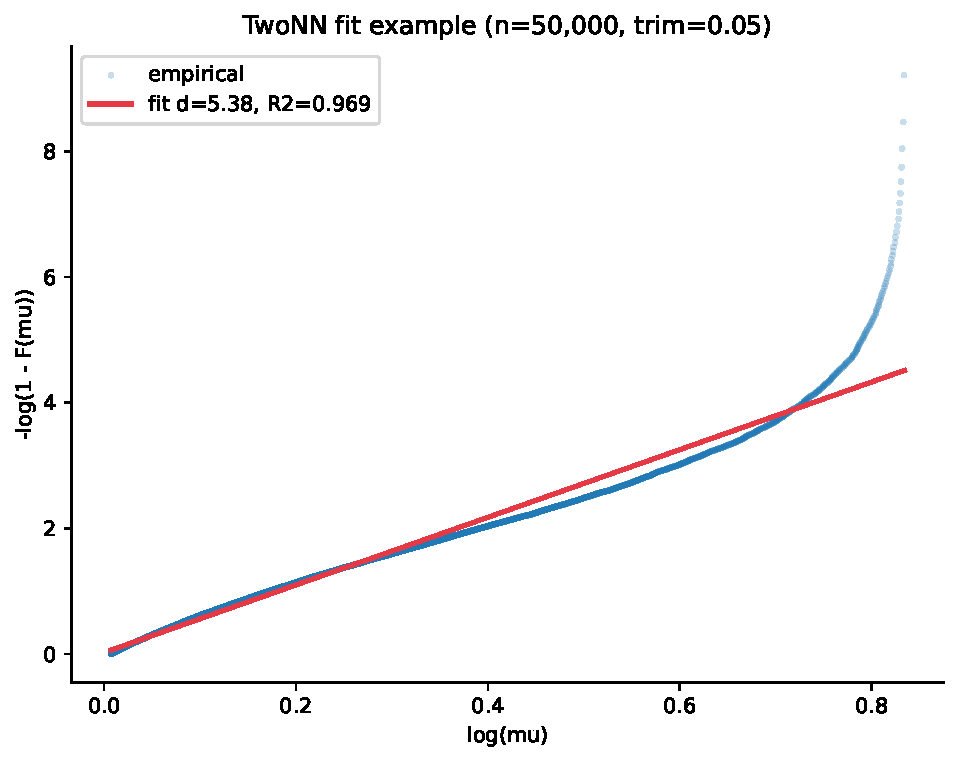
\includegraphics[width=\textwidth]{figures/twonn_fit_example.pdf}
\caption{Ejemplo de ajuste lineal.}
\end{subfigure}
\caption{Diagnósticos de dimensión intrínseca TwoNN después de deduplicación exacta HA+NA. Las estimaciones deben interpretarse como un rango de sensibilidad porque los métodos de dimensión intrínseca basados en vecinos más cercanos se ven afectados por densidad, anisotropía, recorte y efectos de muestra finita.}
\label{fig:twonn}
\end{figure}

\subsection{La estructura temporal es local más que cronológica global}

Aunque las correlaciones temporales globales son débiles, los vecinos latentes más cercanos están mucho más próximos en el tiempo que pares aleatorios emparejados por subtipo después de deduplicación exacta HA+NA (Tabla~\ref{tab:temporal-local}, Figura~\ref{fig:temporal-local}). Para H1N1, la diferencia temporal mediana entre vecinos latentes es 2 meses para $k=5,10,20$, comparada con 42--43 meses para pares aleatorios emparejados por subtipo. Para H3N2, las medianas correspondientes son 2 meses para vecinos latentes y 35 meses para pares aleatorios.

Este resultado apoya coherencia temporal local en la nube de embeddings. No muestra que el espacio latente sea un modelo de pronóstico, ni descarta efectos de densidad de muestreo. Sí indica que la organización molecular observada en las correlaciones de distancia está acompañada por enriquecimiento temporal de corto alcance en vecindarios locales.

\begin{table}[H]
\centering
\caption{Coherencia temporal local de vecinos latentes más cercanos después de deduplicación exacta HA+NA. Las líneas base aleatorias están emparejadas por subtipo y usan el mismo número de comparaciones que el conjunto de vecinos correspondiente.}
\label{tab:temporal-local}
\begin{tabular}{lrrrr}
\toprule
Subtipo & k & mediana NN meses & mediana aleatoria meses & razón \\
\midrule
H1N1 & 5 & 2.00 & 43.00 & 0.047 \\
H1N1 & 10 & 2.00 & 42.00 & 0.048 \\
H1N1 & 20 & 2.00 & 42.00 & 0.048 \\
H3N2 & 5 & 2.00 & 35.00 & 0.057 \\
H3N2 & 10 & 2.00 & 35.00 & 0.057 \\
H3N2 & 20 & 2.00 & 35.00 & 0.057 \\
\bottomrule
\end{tabular}
\end{table}

\begin{figure}[H]
\centering
\begin{subfigure}{0.48\textwidth}
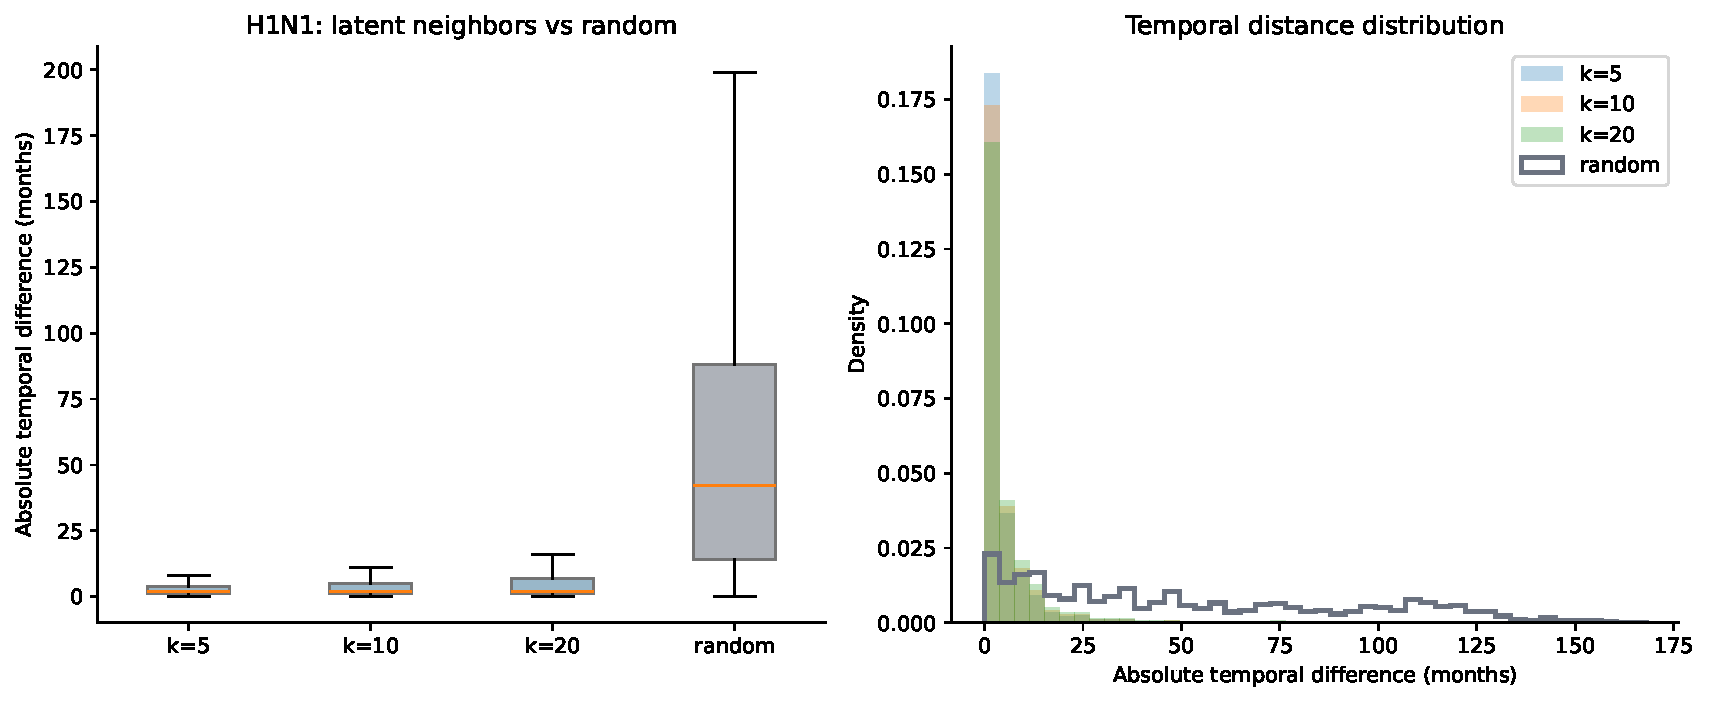
\includegraphics[width=\textwidth]{figures/temporal_local_neighbors_h1n1_dedup.pdf}
\caption{H1N1.}
\end{subfigure}
\begin{subfigure}{0.48\textwidth}
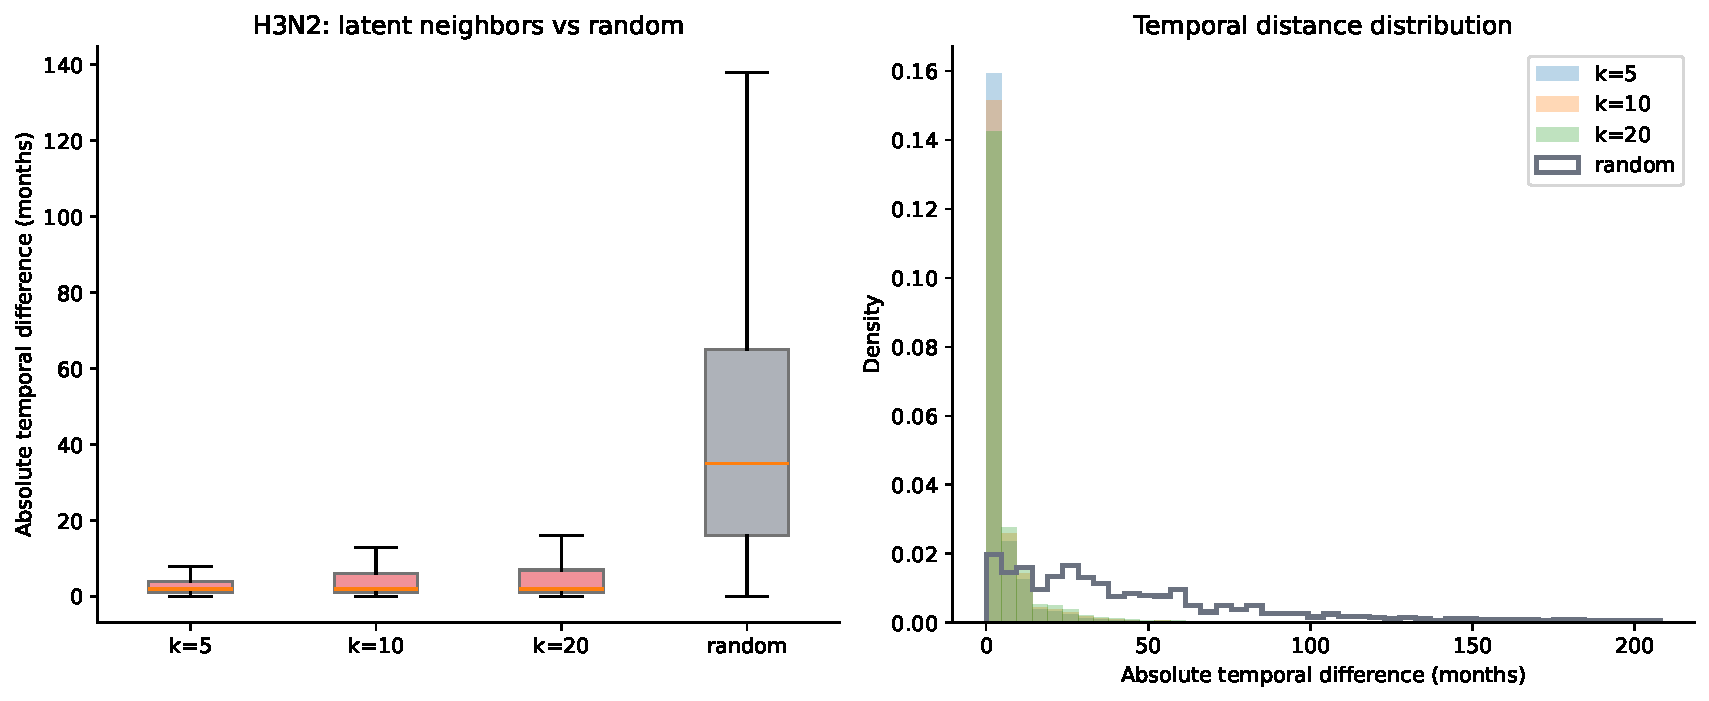
\includegraphics[width=\textwidth]{figures/temporal_local_neighbors_h3n2_dedup.pdf}
\caption{H3N2.}
\end{subfigure}
\caption{Diferencias temporales de vecinos latentes más cercanos frente a líneas base aleatorias emparejadas por subtipo después de deduplicación exacta HA+NA.}
\label{fig:temporal-local}
\end{figure}

\subsection{Controles focalizados de robustez apoyan las principales afirmaciones geométricas}

La deduplicación exacta HA+NA reduce pero no elimina la señal de distancia molecular (Tabla~\ref{tab:robust-spearman}). Después de la deduplicación, las correlaciones de Hamming nucleotídicas HA+NA permanecen altas: 0.8358 para H1N1 y 0.6315 para H3N2. Las correlaciones nucleotídicas solo con NA son más bajas que las correlaciones solo con HA en ambos subtipos, mientras que el proxy nucleotídico combinado HA+NA permanece como el resumen más fuerte de distancia nucleotídica. El proxy simple de sensibilidad HA+NA sobre aminoácidos traducidos también permanece sustancialmente correlacionado con la distancia latente, aunque debe interpretarse con cautela porque no se basa en alineamientos proteicos curados.

\begin{table}[H]
\centering
\caption{Panel focalizado de robustez después de deduplicación exacta HA+NA. Los valores son correlaciones de Spearman con muestreo de pares resumidas a través de las semillas 42, 7 y 123 con 200,000 pares solicitados por subtipo y semilla; las desviaciones estándar reportadas son desviaciones entre semillas, no intervalos de confianza. Las distancias de aminoácidos usan traducción simple en marco 0 y se incluyen solo como proxies de sensibilidad, no como alineamientos proteicos curados.}
\label{tab:robust-spearman}
\begin{tabular}{llrr}
\toprule
Métrica & Subtipo & media $\rho$ & sd $\rho$ \\
\midrule
Distancia temporal & H1N1 & 0.0690 & 0.0031 \\
Distancia temporal & H3N2 & 0.1497 & 0.0017 \\
Hamming nucleotídico HA & H1N1 & 0.8086 & 0.0013 \\
Hamming nucleotídico HA & H3N2 & 0.5883 & 0.0006 \\
Hamming nucleotídico NA & H1N1 & 0.7677 & 0.0010 \\
Hamming nucleotídico NA & H3N2 & 0.5287 & 0.0025 \\
Hamming nucleotídico HA+NA & H1N1 & 0.8358 & 0.0010 \\
Hamming nucleotídico HA+NA & H3N2 & 0.6315 & 0.0015 \\
Proxy HA+NA de aminoácidos traducidos & H1N1 & 0.7563 & 0.0013 \\
Proxy HA+NA de aminoácidos traducidos & H3N2 & 0.6131 & 0.0008 \\
\bottomrule
\end{tabular}
\end{table}

El resultado de vecindarios temporales también es robusto a un control de permutación de etiquetas de fecha (Tabla~\ref{tab:temporal-permutation}). Al mantener fijo el grafo de vecinos latentes pero permutar las etiquetas de índice mensual de colección dentro de subtipo, las diferencias temporales medianas entre vecinos aumentan de 2 meses a 42--43 meses en H1N1 y 35 meses en H3N2, coincidiendo con la línea base aleatoria emparejada por subtipo. Esto apoya la interpretación de que la coherencia temporal local está ligada a las fechas de colección observadas y no solo a la distribución marginal de fechas, bajo este control específico de permutación dentro de subtipo.

\begin{table}[H]
\centering
\caption{Control de permutación de etiquetas de fecha para vecindarios temporales locales después de deduplicación exacta HA+NA. El grafo de vecinos latentes se mantiene fijo y las etiquetas de índice mensual de colección se permutan dentro de subtipo a través de las semillas 42, 7 y 123.}
\label{tab:temporal-permutation}
\begin{tabular}{lrrrr}
\toprule
Subtipo & k & mediana verdadera meses & mediana permutada meses & verdadero/permutado \\
\midrule
H1N1 & 5 & 2.00 & 42.33 & 0.047 \\
H1N1 & 10 & 2.00 & 42.67 & 0.047 \\
H1N1 & 20 & 2.00 & 42.67 & 0.047 \\
H3N2 & 5 & 2.00 & 35.00 & 0.057 \\
H3N2 & 10 & 2.00 & 35.00 & 0.057 \\
H3N2 & 20 & 2.00 & 35.00 & 0.057 \\
\bottomrule
\end{tabular}
\end{table}

\section{Discusión}

Esta auditoría apoya una interpretación cautelosa pero útil de la nube local de embeddings de AntigenLM. El resultado más fuerte es molecular: la distancia euclidiana latente está altamente asociada en rangos con las distancias de Hamming nucleotídicas HA y HA+NA dentro de subtipo. Esto indica que la representación no es simplemente una caja negra de alta dimensión para estos registros; su geometría métrica captura una cantidad sustancial de variación de la secuencia de entrada.

El panel de robustez fortalece esta interpretación dentro de los límites de los controles realizados. Las correlaciones moleculares persisten después de deduplicación exacta HA+NA, y el patrón no se restringe solo a HA: las correlaciones solo con NA también son sustanciales, aunque más bajas que las de HA en este panel. El proxy simple de sensibilidad de aminoácidos traducidos da un resultado cualitativamente similar, aunque sigue siendo menos definitivo que un análisis con alineamiento proteico curado.

Los resultados temporales aclaran qué tipo de estructura evolutiva está presente. La distancia cronológica global está débilmente correlacionada con la distancia latente, lo cual es esperable para una población viral ramificada y muestreada de forma desigual. Sin embargo, los vecindarios locales son temporalmente coherentes después de deduplicación exacta HA+NA. El control de permutación de etiquetas de fecha dentro de subtipo desplaza las diferencias temporales medianas entre vecinos de regreso a valores parecidos a los aleatorios cuando el grafo de vecinos latentes se mantiene fijo, lo que indica que la señal temporal local depende de las etiquetas temporales observadas y no solo de la distribución marginal de fechas de colección. Para futuro modelamiento dinámico, este resultado local es más relevante que la correlación global con el tiempo, porque un modelo de espacio de estados usualmente dependería de transiciones o vecindarios locales y no de tratar todos los pares de años como si estuvieran sobre una sola línea.

El análisis de etiquetas de clado añade una capa de validación cualitativamente distinta. La correlación con distancia de Hamming muestra que las distancias latentes preservan similitud molecular cruda; el enriquecimiento por etiquetas de clado pregunta si los vecindarios locales son coherentes con una anotación evolutivo-taxonómica externa usada en vigilancia de influenza. La respuesta es positiva bajo controles globales emparejados por subtipo y de permutación de etiquetas de clado, especialmente en H3N2, donde la línea base aleatoria emparejada por subtipo es baja porque las etiquetas de clado son más granulares. El control estratificado temporalmente es más sobrio: el enriquecimiento se atenúa cuando los candidatos aleatorios se restringen a meses cercanos de colección, particularmente para H1N1. Esto indica que la coherencia de clado está parcialmente entrelazada con el recambio temporal de periodos dominados por ciertos clados. Por tanto, la interpretación correcta no es que el embedding capture estructura filogenética independiente del tiempo, sino que los vecindarios latentes locales son más coherentes en clado que registros aleatorios del mismo subtipo, incluidos registros muestreados en ventanas temporales comparables.

PCA y TwoNN ofrecen evidencia complementaria de baja estructura efectiva. El PCA muestra que la varianza se concentra en pocas direcciones dominantes, mientras que TwoNN sugiere baja dimensión local bajo razones estandarizadas de vecinos más cercanos. Estos son diagnósticos alentadores para modelamiento reducido, pero no son una prueba matemática de una variedad suave ni de la dimensión correcta para un modelo dinámico posterior.

Los resultados apoyan una interpretación geométrica estrecha y cuidadosamente acotada: los embeddings en caché exhiben organización molecular ($\rho=0.8538$ y 0.6678 para HA+NA), son anisotrópicos y de baja dimensión bajo los diagnósticos evaluados ($n_{95}=3$ global en PCA; estimaciones TwoNN aproximadamente 3.9--5.5 dependiendo del recorte), muestran enriquecimiento temporal local (diferencia mediana entre vecinos de 2 meses frente a 35--43 meses para líneas base aleatorias emparejadas por subtipo) y están localmente enriquecidos para pertenencia a clados de GISAID (precisión@5 de 0.9149 en H1N1 y 0.8609 en H3N2). Estas propiedades no son reproducidas por el control de embeddings aleatorios, el control de permutación de fechas ni el control de permutación de etiquetas de clado, y persisten después de deduplicación exacta HA+NA. Estos hallazgos siguen siendo evidencia a nivel de auditoría: apoyan estructura molecular, dimensional, temporal y de etiquetas de clado en los embeddings en caché, pero no validez antigénica, filogenética, funcional, vacunal ni de pronóstico. Trabajo futuro debe validar estos embeddings contra datos de inhibición de hemaglutinación, distancias filogenéticas y benchmarks de pronóstico prospectivo antes de afirmar relevancia viral-evolutiva o clínica.

\section{Limitaciones}

La limitación más importante es biológica. La distancia de Hamming nucleotídica es un proxy de similitud molecular de secuencia, no un alineamiento curado, una comparación estructural de proteínas ni una medida experimental de distancia antigénica. La distancia de Hamming es útil para una auditoría molecular transparente, pero no captura efectos estructurales de proteína, patrones de conservación, interacciones epistáticas, glicosilación, contexto de unión a receptor ni efectos antigénicos medidos experimentalmente. Este artículo no incluye títulos de ensayos de inhibición de hemaglutinación o neutralización, coordenadas de cartografía antigénica inferidas a partir de datos serológicos, alineamientos curados de secuencias proteicas o anotaciones estructurales, anotación explícita de sitios antigénicos conocidos como el dominio de unión al receptor de HA, distancias filogenéticas inferidas por modelos de alineamiento de máxima verosimilitud o bayesianos, ni mediciones directas de fitness. Por tanto, esta auditoría geométrica no puede establecer similitud antigénica, escape inmune, éxito de clado, validez filogenética cuantitativa, conservación funcional ni relevancia para cepas vacunales. Cualquier uso posterior de estos embeddings para modelamiento de evolución viral, priorización de cepas o interpretación antigénica requiere validación biológica independiente.

El análisis de enriquecimiento por etiquetas de clado tiene limitaciones adicionales. Las anotaciones de clado de GISAID son agrupamientos administrativos/evolutivos basados en criterios filogenéticos, no distancias filogenéticas cuantitativas. Compartir pertenencia a clado no implica igual distancia dentro de un árbol: dos secuencias en el mismo clado pueden diferir sustancialmente en su posición dentro del clado, y dos secuencias en clados distintos pueden seguir siendo cercanas cerca de una frontera. El análisis por tanto evalúa coherencia taxonómica local, no estructura filogenética proporcional a la distancia. La cobertura de anotación de clado también es desigual entre subtipos y años: los registros H1N1 tuvieron 98.38\% de cobertura con clado asignado después de la deduplicación, mientras que los registros H3N2 tuvieron 87.99\%, con baja cobertura de clado H3N2 en los años más tempranos del conjunto. La línea base aleatoria estratificada temporalmente muestra que el enriquecimiento por etiquetas de clado se explica parcialmente por co-ocurrencia temporal de periodos dominados por clados, especialmente en H1N1. Sesgos geográficos, de huésped, laboratorio y composición de linajes en el muestreo de GISAID permanecen sin controlar. Finalmente, los registros \path{unassigned} se excluyeron como valores faltantes; si las secuencias no asignadas son sistemáticamente divergentes, raras o atípicas, su exclusión podría sesgar el análisis hacia secuencias mejor anotadas y más típicas filogenéticamente.

Una segunda limitación se refiere a la validación del análisis de correlación de rangos. La correlación de rangos de Spearman resume asociación global sobre pares muestreados, pero las distancias por pares son inherentemente dependientes: cada registro puede participar en múltiples pares, creando dependencia estructural en el estimador de correlación. Reportamos desviaciones estándar entre semillas de muestreo de pares y, para el control de embeddings aleatorios, entre réplicas de embeddings aleatorios, como resúmenes de sensibilidad más que como intervalos de confianza por bootstrap. La verdadera distribución muestral de $\rho$ bajo dependencia por pares no está capturada por la variación entre semillas. La línea base de embeddings aleatorios demuestra que las principales correlaciones HA+NA no son reproducidas por vectores aleatorios independientes, pero sigue siendo un control negativo simple; no reemplaza un marco completo de validación métrica. Análisis faltantes incluyen pruebas tipo Mantel o Mantel parcial, métricas de correlación de distancias para dependencia no lineal \cite{szekely2007distance}, precisión local de recuperación por $k$ vecinos más cercanos, análisis locales por cuantiles de distancia y métricas de confiabilidad/continuidad para preservación topológica \cite{lee2009quality}. Estos diagnósticos más amplios darían una imagen más completa de qué tan bien las distancias latentes preservan estructura de vecindad molecular más allá de la asociación global de rangos.

El análisis de robustez con aminoácidos traducidos también es limitado. Usa traducción simple en marco 0 de las cadenas nucleotídicas disponibles, mapea codones ambiguos a un símbolo desconocido y descarta codones incompletos terminales. Es un análisis de sensibilidad para evaluar si la señal molecular amplia persiste bajo una representación traducida burda; no es extracción proteica curada, alineamiento múltiple de secuencias, análisis de sitios antigénicos, modelamiento estructural de proteínas ni validación a nivel de proteína. En particular, no resuelve problemas de curación de marco de lectura, péptidos señal, esquemas de numeración, manejo de inserciones/deleciones, regiones antigénicas conocidas de HA/NA ni contexto estructural específico por subtipo. Un análisis más fuerte a nivel proteico requeriría secuencias proteicas HA y NA curadas, comparaciones de residuos conscientes del alineamiento e idealmente conexión con mediciones antigénicas experimentales.

Una tercera limitación concierne la interpretación de dimensión intrínseca. La dimensión efectiva de PCA refleja concentración de varianza, pero puede estar impulsada por anisotropía, agrupamiento por subtipo, desbalance de muestreo, registros duplicados o casi duplicados, o direcciones dominantes inducidas por el modelo, no necesariamente por una variedad biológica suave de baja dimensión. De modo similar, las estimaciones TwoNN pueden verse afectadas por duplicados exactos y casi duplicados, densidad no uniforme, efectos de borde, sesgo de muestra finita, estandarización de coordenadas y nivel de recorte. Eliminamos duplicados exactos HA+NA para TwoNN y análisis locales, pero permanecen casi duplicados y densidad de muestreo desigual. Por tanto, los resultados actuales deben leerse como evidencia de estructura de baja dimensión bajo diagnósticos y decisiones de preprocesamiento específicos, no como una estimación definitiva de dimensión intrínseca. El rango observado, aproximadamente 3.9--5.5 dependiendo del recorte, es en sí mismo evidencia de que la estimación es sensible a supuestos.

Una cuarta limitación importante es el sesgo de vigilancia inherente a secuencias derivadas de GISAID. La intensidad de vigilancia, las prácticas de laboratorios de colección, especies huésped, representación geográfica, protocolos de secuenciación y prácticas de compartición de datos varían entre años, ubicaciones y subtipos. La línea base aleatoria emparejada por subtipo controla por distribuciones marginales de fechas dentro de subtipo, y el control de permutación de etiquetas de fecha pregunta si el enriquecimiento temporal permanece cuando el grafo de vecinos latentes se mantiene fijo pero las fechas se permutan dentro de subtipo. Estos controles reducen dos explicaciones simples, pero no explican confusión por geografía, huésped, intensidad de colección, composición de linajes o ráfagas de muestreo alrededor de brotes. La coherencia temporal local, incluida la diferencia mediana entre vecinos más cercanos de 2 meses, puede reflejar parcialmente agrupamiento de muestras durante campañas de vigilancia, olas pandémicas o brotes locales más que dinámica evolutiva intrínseca de la población viral subyacente. Resolver esta confusión requeriría estratificación por geografía, huésped, linaje o régimen de muestreo, lo cual no se realiza aquí. Por tanto, la señal temporal debe interpretarse cautelosamente como una propiedad del conjunto muestreado y de la representación en caché, no necesariamente como una estimación directa del ritmo evolutivo poblacional.

Finalmente, este análisis no es una reproducción ni validación de la tubería completa de pronóstico de AntigenLM \cite{pei2026antigenlm}. No decodificamos ni generamos secuencias desde los embeddings, no entrenamos un modelo dinámico posterior, no puntuamos mutaciones virales candidatas o estrategias de optimización, no evaluamos desempeño en pronósticos prospectivos posteriores a 2022, no comparamos contra métodos filogenéticos de pronóstico como modelos de fitness o predictores de forma de árbol \cite{luksza2014fitness,neher2014predicting}, ni hacemos benchmark contra selecciones estacionales de cepas vacunales de la OMS. Esta es una auditoría de geometría y enriquecimiento de etiquetas, no una validación de pronóstico, antigénica o funcional. La presencia de organización molecular, baja dimensión efectiva, estructura temporal local y enriquecimiento por etiquetas de clado es una precondición favorable para modelamiento futuro, pero no es evidencia de desempeño suficiente para decisiones clínicas o de salud pública.

\section{Reproducibilidad y disponibilidad de datos}

La tubería local de análisis está basada en scripts. Los embeddings fueron producidos por \path{latent_geometry.py}, las métricas y figuras de datos completos por \path{latent_geometry_full_analysis.py}, y el paquete del artículo por \path{make_paper_1_latent_geometry_full.py}. El panel focalizado de robustez se ejecutó con \path{paper_revision_outputs/run_robustness_panel.py}, el control negativo de embeddings aleatorios con \path{paper_revision_outputs/run_random_embedding_baseline.py}, y el análisis de enriquecimiento por etiquetas de clado con \path{paper_revision_outputs/run_clade_enrichment_analysis.py}. Los resultados agregados primarios se almacenan en \path{results/latent_geometry_full_metrics.json} y se resumen en \path{results/latent_geometry_full_summary.md}; los resultados de robustez se almacenan en \path{paper_revision_outputs/robustness_panel_results.json} y \path{paper_revision_outputs/robustness_panel_summary.md}; los resultados de línea base aleatoria se almacenan en \path{paper_revision_outputs/random_embedding_baseline_results.json} y \path{paper_revision_outputs/random_embedding_baseline_summary.md}; los resultados de enriquecimiento por etiquetas de clado se almacenan en \path{results/gisaid_clade_enrichment_results.json} y \path{results/gisaid_clade_enrichment_summary.md}. Las tablas y figuras del manuscrito se generan desde salidas agregadas y se copian al directorio del artículo.

La redistribución de secuencias crudas y metadatos a nivel de accesión puede estar restringida por los términos de la fuente original de datos. Por esa razón, este manuscrito reporta métricas, conteos, tablas y figuras agregadas en lugar de secuencias completas o metadatos a nivel de accesión. El código y los resultados agregados están disponibles públicamente en \url{https://github.com/cmorregof/latent_geometry}. El repositorio incluye todos los scripts de análisis, salidas JSON agregadas e instrucciones para que usuarios autorizados de GISAID reconstruyan el conjunto procesado y la caché de embeddings usando el checkpoint documentado de AntigenLM (SHA256: \path{6b942a0e2d6af0528a7307ff5754438ad55fdb97390297e9c0f11ffc9803dbff}). La unión de metadatos de clado usó exportaciones locales de GISAID EpiFlu asociadas con \path{EPI_SET_260506bu}; las salidas agregadas de enriquecimiento por etiquetas de clado se redistribuyen, pero la exportación privada de metadatos y la tabla de unión a nivel de accesión no. Cualquier declaración final de disponibilidad de datos también debe seguir los términos aplicables de reconocimiento y uso de datos de GISAID, sin redistribuir secuencias completas restringidas.

\subsection*{Declaración de disponibilidad de datos}

Las secuencias HA/NA crudas de Influenza A derivan de GISAID \cite{shu2017gisaid} y pueden estar sujetas a acuerdos de uso de datos y políticas de reconocimiento de GISAID. Las secuencias completas y los metadatos a nivel de accesión no se redistribuyen en este manuscrito ni en materiales suplementarios. Las salidas agregadas usadas por el manuscrito están disponibles en el repositorio del artículo como archivos JSON y Markdown, incluyendo \path{results/latent_geometry_full_metrics.json} para el análisis primario, \path{paper_revision_outputs/robustness_panel_results.json} para chequeos de robustez deduplicados, \path{paper_revision_outputs/random_embedding_baseline_results.json} para el control negativo de embeddings aleatorios, y \path{results/gisaid_clade_enrichment_results.json} para el análisis de enriquecimiento por etiquetas de clado. El código y los resultados agregados están disponibles públicamente en \url{https://github.com/cmorregof/latent_geometry}. El repositorio incluye todos los scripts de análisis, salidas JSON agregadas e instrucciones para que usuarios autorizados de GISAID reconstruyan el conjunto procesado y la caché de embeddings usando el checkpoint documentado de AntigenLM (SHA256: \path{6b942a0e2d6af0528a7307ff5754438ad55fdb97390297e9c0f11ffc9803dbff}). Los datos de secuencia están sujetos a acuerdos de uso de datos de GISAID. Los usuarios que deseen acceder a las secuencias subyacentes deben solicitar acceso a GISAID y aceptar los términos aplicables. Una lista completa de identificadores de accesión de GISAID para los registros usados en este análisis se proporciona en la Tabla Suplementaria~S1 de acuerdo con los requisitos de reconocimiento de GISAID.

\section{Ética, bioseguridad y uso responsable}

Este trabajo es un análisis de embeddings existentes de secuencias de influenza. No genera secuencias virales, no optimiza mutaciones, no sintetiza constructos, no proporciona protocolos experimentales, no hace recomendaciones vacunales y no asesora decisiones clínicas o de salud pública. Cualquier uso futuro de representaciones aprendidas para pronóstico, priorización de cepas o interpretación antigénica debe evaluarse con validación prospectiva apropiada, revisión de dominio y gobernanza de bioseguridad.

\section{Conclusión}

Presentamos una auditoría geométrica sistemática de embeddings de AntigenLM para 111,756 registros HA/NA de Influenza A. Los resultados muestran que la distancia euclidiana latente se correlaciona fuertemente con proxies nucleotídicos de distancia de secuencia ($\rho=0.8538$ para H1N1 y 0.6678 para H3N2 usando distancia de Hamming HA+NA), mientras que embeddings gaussianos aleatorios normalizados a norma unitaria producen correlaciones cercanas a cero. La nube de embeddings también muestra fuerte concentración lineal de varianza bajo PCA, baja dimensión local de vecinos más cercanos bajo diagnósticos TwoNN y enriquecimiento temporal local respecto a líneas base aleatorias emparejadas por subtipo. Después de deduplicación exacta HA+NA, los vecindarios latentes también están enriquecidos para pertenencia a clados de GISAID: para $k=5$, la precisión de clado es 0.9149 para H1N1 y 0.8609 para H3N2, correspondiente a enriquecimientos de 3.80 y 12.49 veces sobre líneas base aleatorias emparejadas por subtipo. El control de permutación de etiquetas de clado devuelve la precisión a niveles de línea base aleatoria emparejada por subtipo. Las líneas base aleatorias estratificadas temporalmente atenúan la señal, especialmente para H1N1 (1.55 veces en $\pm 6$ meses), mostrando que la coherencia de clado está parcialmente acoplada al recambio temporal de clados pero permanece por encima de la expectativa aleatoria emparejada por tiempo en todas las ventanas evaluadas.

Estos resultados muestran que la nube de embeddings en caché tiene estructura geométrica útil para organización local molecular, temporal y evolutivo-taxonómica bajo los diagnósticos evaluados aquí. Estos hallazgos deben tratarse como precondiciones geométricas y de enriquecimiento de etiquetas favorables para futuro modelamiento probabilístico de la evolución de influenza, no como evidencia de validez antigénica, filogenética, vacunal, de generación de secuencias o de pronóstico. La validación biológica contra ensayos de inhibición de hemaglutinación o neutralización, distancias filogenéticas cuantitativas, controles de muestreo conscientes de geografía/huésped y benchmarks prospectivos posteriores a 2022 sigue siendo esencial antes de afirmar relevancia evolutiva o clínica.

\section*{Agradecimientos}

Agradecemos sinceramente a todos los contribuidores de datos, es decir, a los autores y laboratorios de origen responsables de obtener las muestras, así como a los laboratorios remitentes por generar las secuencias y metadatos y compartirlos mediante la Iniciativa GISAID, en la cual se basa esta investigación.

La base de datos GISAID EpiFlu se describe en Shu y McCauley \cite{shu2017gisaid}: GISAID: Global initiative on sharing all influenza data -- from vision to reality. \emph{Euro Surveillance}. 22(13):30494. DOI: 10.2807/1560-7917.ES.2017.22.13.30494.

Una lista completa de laboratorios contribuidores e identificadores de accesión de secuencia para los registros usados en este análisis, incluidos los registros cubiertos por la exportación local de metadatos \path{EPI_SET_260506bu}, se proporciona en la Tabla Suplementaria~S1, que debe incluirse en el paquete de envío siguiendo las guías de uso de datos de GISAID.

\bibliographystyle{plain}
\bibliography{../papers/paper_1_latent_geometry_full/references}

\end{document}
